\documentclass{article}
% Fifth-draft pilot: conservative compression of the November 14 v4 revision.
% Preserve the v4 section order, numerical results, revision colors, and comments.
% Detailed architecture notation and the training schematic move to Appendix A.
% ICLR review formatting and disclosure sections from archive/main_v3.tex.
% Author annotations remain in the source and are hidden in the PDF.

% Official ICLR 2027 submission template.
% Keep anonymous review mode. Enable only for an accepted camera-ready paper.
\usepackage{iclr2027_conference,times}
% \iclrfinalcopy

\usepackage[utf8]{inputenc} % allow utf-8 input
\usepackage[T1]{fontenc}    % use 8-bit T1 fonts
\usepackage{hyperref}       % hyperlinks
\usepackage{url}            % simple URL typesetting
\usepackage{booktabs}       % professional-quality tables
\usepackage{amsfonts}       % blackboard math symbols
\usepackage{nicefrac}       % compact symbols for 1/2, etc.
\usepackage{microtype}      % microtypography
\usepackage{xcolor} 
% colors
\usepackage{amsmath,amssymb,amsthm,mathrsfs,mathtools,bm}
\usepackage{graphicx}
\usepackage{subcaption}
\usepackage{placeins}

% User writing suggestions are annotations, not instructions to rewrite prose.
\newcommand{\suozhi}[1]{}
\newcommand{\lh}[1]{}
\newcommand{\codexedit}[1]{#1}
\newenvironment{codexrevision}{\begingroup}{\par\endgroup}
% Keep compatibility with existing clean-preview builds.
\ifdefined\hideauthorcomments
    \renewcommand{\suozhi}[1]{}
\fi

% Revisions relative to archive/main_v3.tex: only changed text and numerical
% values are blue; preserved wording remains black. Figures have no revision frames.
\usepackage{etoolbox}
\newcommand{\vfourchange}[1]{{\color{blue}#1}}
\pdfstringdefDisableCommands{\def\vfourchange#1{#1}}
% November 14 smoothing revision: new changes are red; earlier changes stay blue.
\newcommand{\vfourred}[1]{{\color{red}#1}}
\pdfstringdefDisableCommands{\def\vfourred#1{#1}}
\newcommand{\vfourbibitem}[2][]{%
    \par\color{black}% finish the preceding reference before changing color
    \vfouroriginalbibitem[#1]{#2}%
    \ifstrequal{#2}{hersbach2020era5}{\color{blue}}{}%
    \ifstrequal{#2}{subich2025spectral}{\color{red}}{}%
}
\AtBeginEnvironment{thebibliography}{%
    \let\vfouroriginalbibitem\bibitem
    \let\bibitem\vfourbibitem
}

\title{GraphCast--Mamba: Learning Non-Markovian Corrections for Weather Forecasting}


% The \author macro works with any number of authors. There are two commands
% used to separate the names and addresses of multiple authors: \And and \AND.
%
% Using \And between authors leaves it to LaTeX to determine where to break the
% lines. Using \AND forces a line break at that point. So, if LaTeX puts 3 of 4
% authors names on the first line, and the last on the second line, try using
% \AND instead of \And before the third author name.


\author{
}



% V5 review layer. v5.tex shows changes; v5_clean.tex hides this layer.
\usepackage[normalem]{ulem}
\definecolor{vfiveDeleted}{RGB}{150,45,45}
\definecolor{vfiveAdded}{RGB}{0,105,65}
\newif\ifvfivechanges
\ifdefined\vfiveclean\vfivechangesfalse\else\vfivechangestrue\fi
% Clean view: retain revision highlighting in blue, with all deletions hidden.
\ifvfivechanges\else\colorlet{red}{blue}\fi
\newcommand{\vfiveidentity}[1]{#1}
\DeclareRobustCommand{\vfiveadded}[1]{\ifvfivechanges{\color{vfiveAdded}%
  \let\vfourchange\vfiveidentity\let\vfourred\vfiveidentity#1}\else{\color{blue}%
  \let\vfourchange\vfiveidentity\let\vfourred\vfiveidentity#1}\fi}
\pdfstringdefDisableCommands{\def\vfiveadded#1{#1}\def\sout#1{#1}}
\DeclareRobustCommand{\vfiveRone}[1]{\ifvfivechanges{\color{vfiveDeleted}\sout{#1}}\,\fi\vfiveadded{R1}}
\pdfstringdefDisableCommands{\def\vfiveRone#1{R1}}
\DeclareRobustCommand{\vfivewordchange}[2]{\ifvfivechanges{\color{vfiveDeleted}\sout{#1}}\,\fi\vfiveadded{#2}}
\pdfstringdefDisableCommands{\def\vfivewordchange#1#2{#2}}

\begin{document}

\maketitle
\ifvfivechanges
\begin{center}\small\textit{V5 review copy: \sout{struck text} is removed or replaced; \textcolor{vfiveAdded}{green text} is the replacement. Moves to Appendix A.2 are labelled. Compile v5\_clean.tex for the page-limit view.}\end{center}
\fi


\begin{abstract}
Unresolved atmospheric processes can introduce history dependence beyond the short input windows used by many weather forecasting models. We introduce GraphCast--Mamba, which augments a frozen, pretrained \(1^\circ\) GraphCast backbone with a trainable correction branch combining graph message passing and Mamba layers. The branch retains a temporal memory state across successive six-hour forecast steps, learning corrections informed by context beyond GraphCast's two-frame input. Training is confined to the correction branch, using ERA5 data from 2015--2021. After 2,500 optimizer updates, including warm-up, \vfourchange{five independent retrainings of the selected configuration reduce GraphCast loss (normalized weighted mean-squared error) by $14.17\%\pm0.43$ percentage points over the full ten-day forecast and by $21.03\%\pm0.75$ percentage points at day 10, evaluated on 122 initializations in 2023; uncertainties are sample standard deviations across training seeds. The original selected checkpoint reduces day-10 root-mean-square error (RMSE) by 7.09--14.60\% across all 11 evaluated variable groups. A matched reset-trained control supports a contribution from persistent memory for the tested training realization.} These results \vfourchange{show} broad improvements through a short correction-training schedule while retaining the pretrained backbone.

\end{abstract}



\section{Introduction}

{Learned global weather models produce skillful forecasts from one or a few recent atmospheric states~\citep{bi2023pangu,lam2023graphcast,chen2023fuxi}. GraphCast, for example, uses two states six hours apart to predict the next state. These inputs provide only a partial description of the atmosphere: they contain a limited set of variables at finite spatial resolution, while unresolved processes can still influence their evolution. The history of the resolved state may carry information about these influences that a short input window does not capture.}

{This is a familiar closure problem in turbulent-flow modeling. Resolving the smallest dynamically active scales is computationally costly~\citep{yang2021grid}, so practical models must account for their effects on the resolved scales. A common approach uses approximate dissipative closures, such as eddy viscosity or hyperviscosity, to represent transfer to unresolved scales. These closures can reproduce selected aspects of the flow, but their accuracy depends on the quantity and scale of interest. For example, in forced two-dimensional turbulence, viscous, hyperviscous, and Leith closures can approximate enstrophy transfer, whereas the Smagorinsky closure dissipates enstrophy at the wrong scales~\citep{pietarila2013closures}. Resolution studies provide a related caution: mean dissipation and enstrophy can be nearly converged while higher-order moments of velocity gradients, dissipation, and enstrophy, together with distribution tails, remain substantially underestimated~\citep{DonzisResolutionEffects}. Reproducing bulk statistics therefore does not ensure accurate fluctuations or extreme events.}

{A complementary approach allows the closure to depend on the history of the resolved state. Unresolved variables have their own dynamics, so their influence need not be determined by the current resolved variables alone; past observations can contain information about those hidden degrees of freedom. The Mori--Zwanzig formalism makes this explicit: eliminating unresolved variables generally yields an instantaneous term, a history-dependent memory term, and a term associated with unresolved initial conditions, even when the full dynamics are Markovian~\citep{YenTingLinMZ2021,de2026data}. Retaining the memory contribution leads to a \emph{non-Markovian} closure, in which the resolved evolution depends on past states as well as the present one. This motivates persistent temporal memory as a mechanism for representing unresolved influences that an instantaneous dissipative approximation may miss.}

{Evidence from learned partial differential equation (PDE) models supports this motivation. Memory Neural Operator (MemNO), which combines a neural operator with a structured state-space sequence (S4) layer, improves predictions from coarse or noisy observations~\citep{buitrago2025memory}. Here, we ask whether retaining temporal context beyond GraphCast's two-frame input improves forecast corrections when the correction architecture and parameter count are held fixed.}


{To investigate this question, we introduce GraphCast--Mamba, which augments a frozen pretrained $1^\circ$ GraphCast backbone with a trainable correction branch combining graph message passing and Mamba layers~\citep{lam2023graphcast,gu2023mamba}. Graph message passing exchanges spatial information, while Mamba retains temporal context across successive six-hour forecast steps. The branch adds a history-dependent correction to each backbone forecast, and the corrected forecast supplies the next input. Only the correction branch is trained.}

Our principal experiment trains the correction on ERA5 data from 2015--2021\vfourchange{, selects the model on 32 forecast initializations from the 2022 development set,} and evaluates ten-day forecasts on \vfourchange{122 initializations in 2023} at $1^\circ$ resolution. This experiment tests the benefit of correction for one pretrained backbone at a fixed resolution. Its dependence on resolution and transfer to other forecasters remain open questions.

Our contributions are threefold.
\begin{itemize}
    \item \textbf{A temporal-memory correction model.} GraphCast--Mamba combines spatial message passing with temporal Mamba layers in a separate Mamba correction branch, extending the predictor's temporal context while keeping the pretrained GraphCast backbone frozen.
    \item \textbf{Evidence for a contribution from temporal memory.} \vfourchange{A matched control trained and evaluated without persistent temporal memory uses the same architecture, parameter count, and optimization schedule. Retaining memory improves ten-day GraphCast loss reduction by $5.26$ percentage points (pointwise paired 95\% confidence interval: $4.70$--$5.86$) for this training realization.}
    \item \vfourchange{\textbf{Broad improvements and training-seed replication.} Five independent retrainings reduce ten-day GraphCast loss by $14.17\%\pm0.43$ percentage points and day-10 loss by $21.03\%\pm0.75$ percentage points (mean $\pm$ sample SD). For the original selected checkpoint, day-10 RMSE decreases by $7.09$--$14.60\%$ across all 11 evaluated variable groups.}
\end{itemize}

\begingroup
\section{Related Work}
\label{sec:related_work}

\begin{figure}[!tp]
    \centering
    \begin{subfigure}{\linewidth}
        \centering
        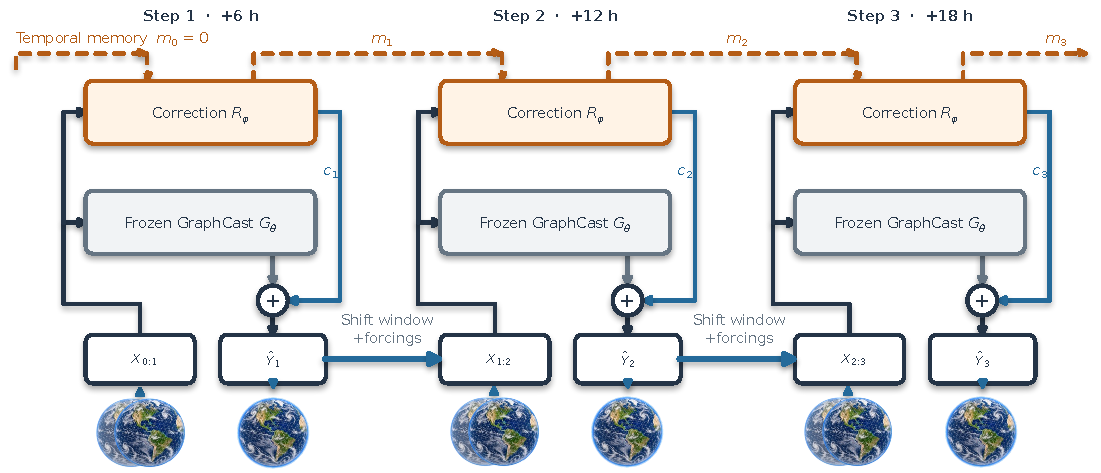
\includegraphics[width=0.93\linewidth]{arxiv_pics/fig1_GC_mamba.pdf}
        \caption{Autoregressive rollout over three six-hour steps. {Each GraphCast--Mamba forecast advances the two-frame input window; dashed orange arrows carry the temporal memory state}, initialized here with $m_0=0$.}
        \label{fig:GC_Mamba_rollout}
    \end{subfigure}
    \par\smallskip
    \begin{subfigure}{\linewidth}
        \centering
        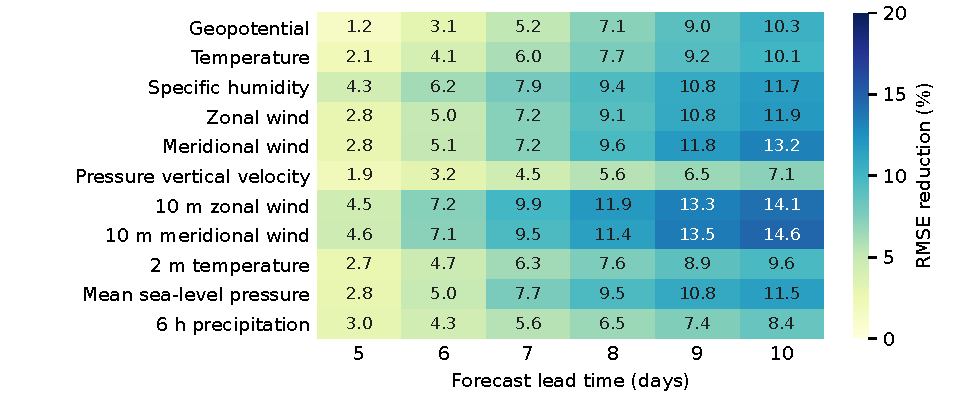
\includegraphics[width=0.93\linewidth]{arxiv_pics/fig1_improvement.pdf}
        \caption{{Variable-group RMSE reductions at days 5 through 10.}}
        \label{fig:breadth_7yr}
    \end{subfigure}
    \par\smallskip
    \begin{subfigure}{\linewidth}
        \centering
        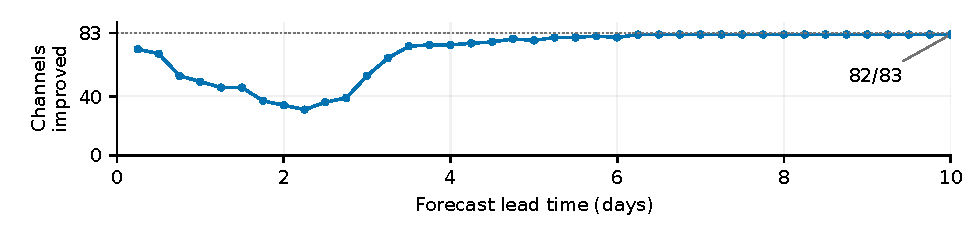
\includegraphics[width=0.93\linewidth]{arxiv_pics/fig1_channel_coverage.pdf}
        \caption{{Channel scores: channels with lower RMSE than GraphCast at each six-hour lead.}}
        \label{fig:coverage_7yr}
    \end{subfigure}
    \caption{\vfourchange{GraphCast--Mamba: temporal-memory correction and forecast-skill overview. Panel (a) shows forecast feedback and memory carry. Panels (b,c) use the original selected checkpoint: (b) gives variable-group RMSE reductions relative to its paired GraphCast baseline; (c) counts channels with lower RMSE, out of 83. These are single-checkpoint aggregate results without channel-wise significance tests. Section~\ref{sec:eval_protocol} defines the protocol and aggregation.}}
    \label{fig:GC_Mamba}
\end{figure}

\begin{figure}[!htbp]
    \centering
    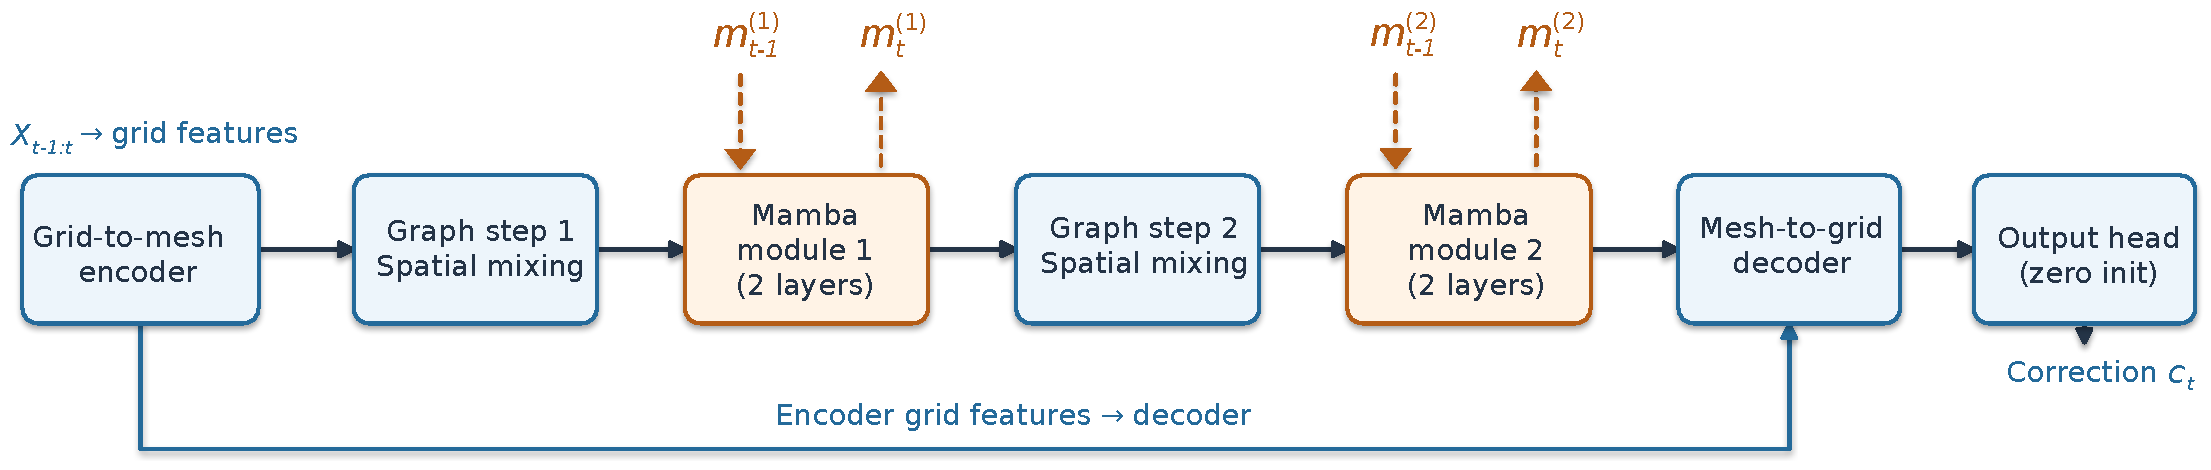
\includegraphics[width=\linewidth]{arxiv_pics/fig2_correction_branch.pdf}
    \caption{{Trainable Mamba correction branch.} Two graph message-passing steps each feed a two-layer Mamba module, followed by decoding and an output head initialized to zero. {The frozen GraphCast backbone forecast $G_\theta(X_t)$ is combined with the learned forecast correction $c_t$ to produce $\hat{Y}_t$. The Mamba correction branch has separate parameters and a temporal memory state $m_t$}, comprising the SSM states and causal-convolution caches of its four Mamba layers.}
    \label{fig:GC_Mamba_correction}
    \vspace{-10pt}
\end{figure}

Our work connects three lines of research: memory-based modeling of partially observed dynamics, temporal memory in weather forecasting, and learned corrections to existing predictors.

\paragraph{Memory and learned closures in reduced dynamics.}
When only part of a dynamical system is resolved, the evolution of the retained variables can depend on their history, as described by the Mori--Zwanzig formalism~\citep{YenTingLinMZ2021}. Motivated by this connection, MemNO combines Fourier neural operators with S4 memory for coarse or noisy PDE observations~\citep{buitrago2025memory}; SS-NO combines spatial state-space operators with temporal memory~\citep{koren2025ssno}. Memory also enters learned corrections to imperfect dynamics: \citet{gupta2021neuralclosures} augment reduced models with neural delay differential equations, while \citet{levine2022modelerror} develop a framework for learning both memoryless and memory-dependent model error. These studies motivate using temporal context to represent effects missing from a predictor's resolved state. Our experiments assess the predictive value of retained context without identifying a physical memory kernel.

\paragraph{Temporal memory in weather forecasting.}
Recurrent weather models already retain information across forecast steps. SwinRNN carries hidden features through global forecasts, while SwinVRNN adds learned perturbations for ensemble prediction~\citep{hu2023swinvrnn}; SwinRDM couples recurrent forecasts with diffusion super-resolution~\citep{chen2023swinrdm}. For radar nowcasting, GauMamba combines Mamba processing with gated recurrent unit (GRU) memory to predict evolving Gaussian representations~\citep{wang2025gaumamba}. These models establish temporal memory as a forecasting mechanism. Our architecture places memory in a separate correction branch: Mamba processes time at each mesh node, graph message passing exchanges spatial information, and the pretrained GraphCast backbone remains frozen.

\paragraph{Learned forecast corrections.}
Learning corrections provides a way to improve an existing predictor while retaining its forecast model. $\delta$-Adapter learns input adjustments and output residual corrections around frozen time-series forecasters~\citep{liang2026forecast}. In numerical weather prediction, \citet{chen2022correcting} learn state-dependent corrections from analysis increments and apply them during FV3-GFS integration. Solver-in-the-Loop trains corrections through differentiable solver rollouts, accounting for their effects on subsequent states~\citep{um2020solver}. These approaches establish both frozen-model adaptation and correction during model integration. For our weather predictor, the remaining question is whether a correction benefits from temporal context beyond the backbone's two-frame input.

These precedents motivate our investigation of persistent temporal memory in a correction branch for a frozen pretrained global weather model. Our experiments compare corrections with and without retained state using the same architecture and parameter count.
\par
\endgroup


\section{Method: A hybrid GraphCast--Mamba architecture}


\ifvfivechanges
\par\begingroup\color{vfiveDeleted}\noindent
\sout{We study whether a temporal memory state improves forecasts beyond the finite input history supplied to the frozen GraphCast backbone. GraphCast uses two successive atmospheric states as input; its forecast is Markovian with respect to this augmented state. Figure~\mbox{\ref{fig:GC_Mamba_rollout}} shows how the Mamba correction branch corrects each GraphCast backbone forecast and carries its temporal memory state across successive six-hour steps. The GraphCast--Mamba forecast advances the meteorological input window, while the temporal memory state retains information from the preceding trajectory. Figure~\mbox{\ref{fig:GC_Mamba_correction}} details how graph message passing mixes information across mesh nodes and Mamba updates memory independently at each node. This introduces history dependence relative to the baseline input representation.}
\par\endgroup
\fi
\vfiveadded{We study whether a temporal memory state improves forecasts beyond GraphCast's two-frame input, with respect to which the backbone is Markovian. Figure~\ref{fig:GC_Mamba_rollout} shows corrected forecast feedback and memory carry; Figure~\ref{fig:GC_Mamba_correction} shows spatial message passing and temporal Mamba updates at each mesh node. This introduces history dependence relative to the baseline input representation.}

\subsection{{Architecture}}

\paragraph{{GraphCast backbone}}
\ifvfivechanges
\par\begingroup\color{vfiveDeleted}\noindent
\sout{The frozen GraphCast backbone uses a pretrained checkpoint and also serves as the standalone forecast baseline. This graph neural network operates on a latitude--longitude grid and an auxiliary mesh, with graph $\mathcal{G}(\mathcal{V}^{\textrm{G}},\mathcal{V}^{\textrm{M}},\mathcal{E}^{\textrm{G2M}},\mathcal{E}^{\textrm{M}},\mathcal{E}^{\textrm{M2G}})$. The vertices $\mathcal{V}^{\textrm{G}}$ represent the meteorological grid and $\mathcal{V}^{\textrm{M}}$ the mesh. Encoding uses grid-to-mesh edges $\mathcal{E}^{\textrm{G2M}}$, followed by $N=16$ graph message-passing steps over $\mathcal{E}^{\textrm{M}}$ and decoding over mesh-to-grid edges $\mathcal{E}^{\textrm{M2G}}$. Latent node features have width $W_{\textrm{GC}}=512$. The mesh provides a more compact representation for spatial processing than the meteorological grid.}
\par\endgroup
\fi
\vfiveadded{The frozen pretrained GraphCast backbone also serves as the standalone baseline. It encodes the latitude--longitude grid onto an auxiliary mesh, applies 16 graph message-passing steps with width-$512$ node features, and decodes back to the meteorological grid. Appendix~\ref{app:architecture_details} gives the graph notation and implementation details.}

\paragraph{{Mamba correction branch: temporal memory on the mesh.}}
The Mamba correction branch uses Mamba~\citep{gu2023mamba} to process forecast time independently at each mesh node, with spatial exchange handled by graph message passing. Each layer normalizes the width-$512$ mesh features, projects them into a $d_{\mathrm{inner}}$-dimensional temporal representation, and projects its output back to the mesh width through a residual connection. We use $d_{\mathrm{inner}}=16$. Across autoregressive forecast calls, each layer retains both its {state-space model (SSM) state} and its three-token causal-convolution cache separately for each batch element and mesh node.

\ifvfivechanges
\par\begingroup\color{vfiveDeleted}\noindent
\sout{Our model uses an SSM state dimension of $16$ per inner channel, a causal convolution width of $4$, a rank-$32$ projection for the step-size parameter $\Delta_t$, and one shared group of input-dependent $B_t,C_t$ coefficients. Additional studies examine $d_{\mathrm{inner}}=32$. The memory-reset controls in Section~\mbox{\ref{sec:memory_ablation}} use $d_{\mathrm{inner}}=16$ and one shared $B,C$ group to test the contribution of temporal memory.}
\par\endgroup
\fi
\vfiveadded{The memory-reset controls in Section~\ref{sec:memory_ablation} use the same architecture; further layer dimensions are given in Appendix~\ref{app:architecture_details}.}


\paragraph{An additive correction with temporal memory.}
Let $X_t$ denote the two-frame meteorological input (shown as $X_{t-1:t}$ in the diagrams) and the associated forcings. Forecast calls are indexed from $t=1$; $\hat{Y}_t$ denotes the next-state forecast produced by call $t$. The temporal memory state $m_t$ collects the SSM states and causal-convolution caches of all Mamba layers. As shown in Figure~\ref{fig:GC_Mamba_rollout}, {GraphCast--Mamba combines the frozen GraphCast backbone $G_\theta$ with the trainable Mamba correction branch $R_\phi$, whose output $c_t$ is the forecast correction}:
\vspace{-4pt}
\begin{equation}
    (c_t,m_t)=R_\phi(X_t,m_{t-1}),
    \qquad
    \hat{Y}_t=G_\theta(X_t)+c_t,
    \qquad \theta\ \text{fixed}.
    \label{eq:additive_correction}
\end{equation}
\ifvfivechanges
\par\begingroup\color{vfiveDeleted}\noindent
\sout{The Mamba correction branch in Figure~\mbox{\ref{fig:GC_Mamba_correction}} has its own grid-to-mesh encoder, mesh processor, and mesh-to-grid decoder. It receives the same meteorological inputs as the GraphCast backbone and uses separate parameters throughout. Its mesh processor uses two graph message-passing steps, each followed by a two-layer Mamba module, giving four recurrent layers in total. Encoder grid features are also passed directly to the decoder. Suppressing this grid-feature connection in the notation, the mesh-processing path is}
\par\endgroup
\fi
\ifvfivechanges
\par\begingroup\color{vfiveDeleted}
\noindent\textit{Detailed equations moved to Appendix A.2.}
\begin{gather*}
\text{\sout{\ensuremath{L_t^{(0)} = \operatorname{Encode}_\phi(X_t),}}}\\
\text{\sout{\ensuremath{\widetilde{L}_t^{(k)} = \operatorname{GNN}^{(k)}_\phi(L_t^{(k-1)}),}}}\\
\text{\sout{\ensuremath{(L_t^{(k)},m_t^{(k)}) =\operatorname{MambaModule}^{(k)}_\phi (\widetilde{L}_t^{(k)},m_{t-1}^{(k)}),\qquad k=1,2,}}}\\
\text{\sout{\ensuremath{c_t = \operatorname{Decode}_\phi(L_t^{(2)}).}}}
\end{gather*}
\endgroup
\fi
\ifvfivechanges
\par\begingroup\color{vfiveDeleted}\noindent
\sout{Each Mamba module contains two residual Mamba layers; $m_t^{(k)}$ comprises their SSM states and causal-convolution caches. The output head is initialized to zero, so the initial GraphCast--Mamba forecast equals the GraphCast backbone forecast. During autoregressive forecasting, the oldest input frame is dropped, the GraphCast--Mamba forecast $\hat{Y}_t$ is appended, and the known forcings are updated to form $X_{t+1}$. The temporal memory state is passed separately to the next correction-branch call. The cold-start rollout illustrated in Figure~\mbox{\ref{fig:GC_Mamba_rollout}} begins with $m_0=0$ and retains the updated temporal memory state thereafter.}
\par\endgroup
\fi
\vfiveadded{The Mamba correction branch has its own grid-to-mesh encoder, mesh processor, and mesh-to-grid decoder. It receives the same meteorological inputs as the backbone and uses separate parameters throughout. Two graph message-passing steps each feed a two-layer Mamba module, giving four recurrent layers. Encoder grid features also pass directly to the decoder. Appendix~\ref{app:architecture_details} gives the corresponding equations. During forecasting, the oldest input frame is dropped, the corrected forecast $\hat{Y}_t$ is appended, and known forcings are updated to form $X_{t+1}$. The temporal memory state starts at $m_0=0$ and is carried separately between forecast calls.}


\subsection{Training}
\label{sec:training}
\paragraph{Initialization and trainable parameters.}
The Mamba correction branch inherits pretrained spatial weights and uses a zero-initialized output head, so the initial GraphCast--Mamba forecast matches the GraphCast backbone forecast. We train all correction-branch parameters $\phi$ on ERA5 2015--2021 while keeping the separate GraphCast backbone parameters $\theta$ frozen.

\paragraph{Training segments and memory carry.}
\ifvfivechanges
\par\begingroup\color{vfiveDeleted}\noindent
\sout{We divide the training sequence into contiguous segments of 96 six-hour steps (24 days), each processed as four consecutive 24-step windows (Figure~\mbox{\ref{fig:training_segments}}). The temporal memory state, comprising both the SSM states and causal-convolution caches, starts at zero for each segment and is carried through all 96 steps. Each window begins with a four-step teacher-forced prefix (ERA5 inputs), followed by 20 feedback-conditioned forecast steps that use the GraphCast--Mamba forecast as feedback. Meteorological inputs therefore return to ERA5 at the start of each window, while the correction branch retains the preceding window's temporal memory state. Gradients propagate through the temporal memory state within a window; at its end, the state is carried forward with its gradient detached. Gradients are also stopped through the meteorological feedback.}
\par\endgroup
\fi
\ifvfivechanges
\par\begingroup\color{vfiveDeleted}
\noindent\textit{Moved to Appendix A.2; original placement shown below.}\par
\begin{center}
    \centering
    \normalsize
    \[
    m_{\mathrm{init}}=0\;\longrightarrow\;
    \underbrace{
      \boxed{1{:}24}
      \xrightarrow{\mathrm{sg}}\boxed{25{:}48}
      \xrightarrow{\mathrm{sg}}\boxed{49{:}72}
      \xrightarrow{\mathrm{sg}}\boxed{73{:}96}
    }_{\text{one segment: memory carried through 96 steps}}
    \xrightarrow{\mathrm{reset}}\;m_{\mathrm{init}}'=0
    \]
    \captionof*{figure}{\sout{Memory carry during training. Boxes show the four 24-step windows of one segment. The arrows marked $\mathrm{sg}$ carry the SSM states and causal-convolution caches unchanged across window boundaries while stopping their gradients. Both are reset for the next segment.}}
    
\end{center}

\par\endgroup
\fi
\vfiveadded{We divide training into segments of 96 six-hour steps (24 days), processed as four consecutive 24-step windows. Both the SSM states and causal-convolution caches start at zero for each segment and are carried through all 96 steps. Each window begins with four teacher-forced steps using ERA5 inputs, followed by 20 steps using corrected forecasts as feedback. Meteorological inputs return to ERA5 at each window boundary, while temporal memory is retained with its gradient detached. Gradients propagate through memory within each window and are stopped through meteorological feedback. Figure~\ref{fig:training_segments} in Appendix~\ref{app:architecture_details} illustrates this procedure.}

\paragraph{Training loss.}
At each step, the forecast correction is supervised against the residual target $r_t=Y_t-G_\theta(X_t)$, where $Y_t$ is ERA5 truth and $X_t$ is the current input. Since $c_t-r_t=\hat{Y}_t-Y_t$, this minimizes the {GraphCast loss} $\ell_{\mathrm{GC}}$ of the GraphCast--Mamba forecast. We average the loss over all $H=24$ steps, including the teacher-forced prefix, and the $B$ batch elements:
\begin{equation}
    \mathcal{J}(\phi)
    =\frac{1}{BH}\sum_{b=1}^{B}\sum_{k=1}^{H}
      \ell_{\mathrm{GC}}(\hat{Y}_{b,k},Y_{b,k}).
    \label{eq:training_objective}
\end{equation}
Appendix~\ref{app:training_loss} gives the full loss definition and weights.

\paragraph{Training schedule.}
We train with AdamW for 2,000 post-warm-up updates after a 500-update warm-up, or 2,500 optimizer updates in total. The evaluated model uses stochastic weight averaging (SWA); Appendix~\ref{app:training} \vfourchange{provides the complete training configuration, model-selection procedure, and computational costs.}


\section{Results}
\label{sec:numerical}

\ifvfivechanges
\par\begingroup\color{vfiveDeleted}\noindent
\sout{We evaluate whether GraphCast--Mamba, with its correction branch trained on seven years of ERA5 data (2015--2021), improves on the frozen GraphCast backbone forecasts, how broadly the gains extend across the atmospheric state, and whether temporal memory contributes beyond the correction branch's additional capacity. To assess the latter, we compare against a matched control trained and evaluated with memory reset at every step.}
\par\endgroup
\fi
\vfiveadded{We evaluate forecast accuracy, the breadth of improvement across the atmospheric state, and the contribution of temporal memory using a matched reset-trained control.}

\subsection{Evaluation protocol and metrics}
\label{sec:eval_protocol}


\begin{figure}[!t]
    \centering
    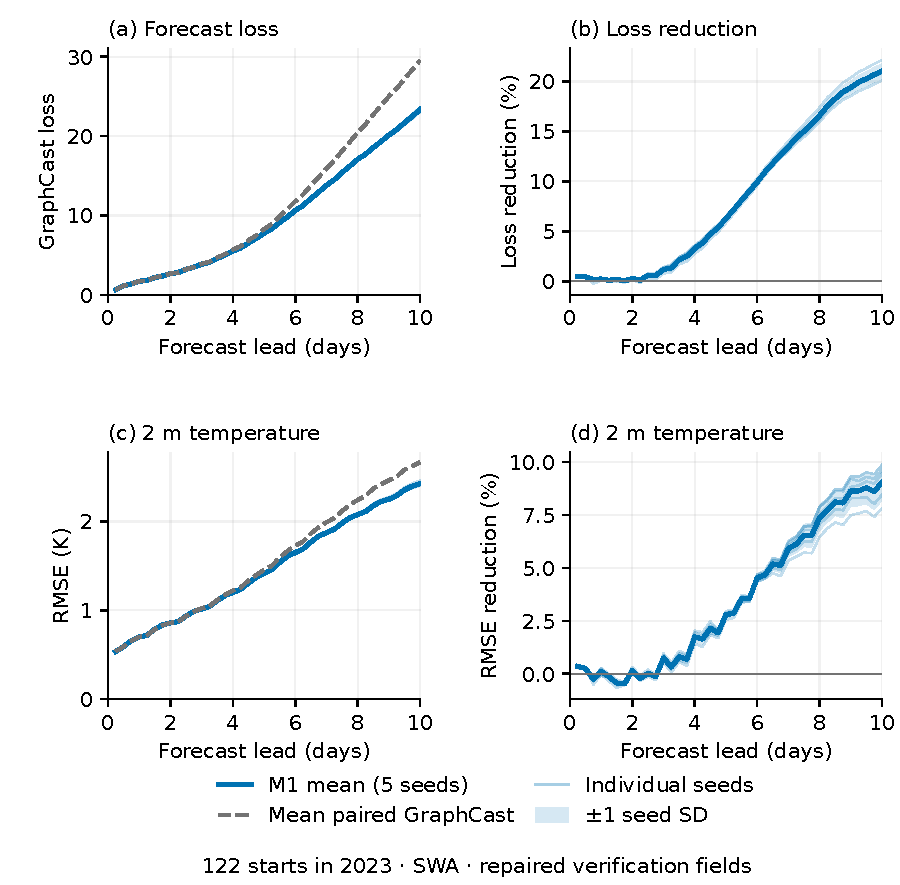
\includegraphics[width=0.8\linewidth]{arxiv_pics/fig3_forecast_skill_v5_seeds.pdf}
    \ifvfivechanges
\caption*{\color{vfiveDeleted}\sout{Five-seed replication on 122 forecast initializations in 2023. Top: exact GraphCast loss and its reduction. Bottom: $2$\,m temperature RMSE and its reduction. Thin curves show independent retrainings with seeds 22--26; the thick curve and shading show their mean and one sample SD, not a confidence interval or a forecast ensemble. Each seed uses its own repeated public GraphCast baseline. Losses and squared physical errors are pooled over dates before ratios and square roots; seed scores are then summarized. All runs use the selected $K=20$, $d_{\mathrm{inner}}=16$ configuration and four-checkpoint SWA (Appendix~\mbox{\ref{app:seed_replication}}).}}
\fi
\caption{\vfiveadded{\vfourchange{Five-seed replication on 122 initializations in 2023. Top: exact GraphCast loss and its reduction. Bottom: $2$\,m temperature RMSE and its reduction. Thin curves show seeds 22--26; the thick curve and shading show their mean and one sample SD, not a confidence interval or forecast ensemble. Each seed uses its own repeated public GraphCast baseline, with errors pooled before ratios and square roots. All runs use $K=20$, $d_{\mathrm{inner}}=16$ and four-checkpoint SWA (Appendix~\ref{app:seed_replication}).}}}
    \label{fig:res1_forecast}
\end{figure}

\ifvfivechanges
\par\begingroup\color{vfiveDeleted}\noindent
\sout{The principal experiments use GraphCast--Mamba with the original pretrained $1^\circ$ GraphCast backbone and the Mamba correction branch trained in Section~\mbox{\ref{sec:training}}. The original checkpoint, denoted M1, was selected among six learning-rate arms on 32 initializations from the 2022 development set (Appendix~\mbox{\ref{sec:training_sensitivity}}) and fixed for evaluation on 122 initializations at 00\,UTC every third day from 1 January to 30 December 2023, at 40 six-hour leads from 6 to 240\,h. M1 supplies the variable-group, channel-coverage, and common-grid results. Figure~\mbox{\ref{fig:res1_forecast}} instead reports five fresh retrainings of its fixed configuration on the same forecast dates; they do not include the original checkpoint. Appendix~\mbox{\ref{app:seed_replication}} distinguishes their provenance and verification-data repairs.}
\par\endgroup
\fi
\vfiveadded{The principal experiments use the pretrained $1^\circ$ GraphCast backbone. \vfourchange{We denote our principal GraphCast--Mamba model by \textbf{M1}: the selected SWA checkpoint trained and evaluated with persistent temporal memory. M1 was selected among six learning-rate arms on 32 initializations from the 2022 development set (Appendix~\ref{sec:training_sensitivity}), then evaluated on 122 initializations at 00\,UTC every third day from 1 January to 30 December 2023, at 40 six-hour leads from 6 to 240\,h. M1 supplies the variable-group, channel-coverage, and common-grid results. Figure~\ref{fig:res1_forecast} reports five fresh retrainings of its fixed configuration on the same dates, excluding M1 (provenance and verification-data repairs: Appendix~\ref{app:seed_replication}).}}

\ifvfivechanges
\par\begingroup\color{vfiveDeleted}\noindent
\sout{Each forecast takes two ERA5 states as input. GraphCast--Mamba initializes the temporal memory state to zero, and advances for ten days using its own predictions as feedback. GraphCast--Mamba feeds back its full prediction, while GraphCast follows an independent uncorrected trajectory. Stateful models retain their updated temporal memory state between steps; the controls without persistent temporal memory reset it at every step.}
\par\endgroup
\fi
\vfiveadded{Each forecast starts from two ERA5 states and advances for ten days using its own predictions as feedback. GraphCast--Mamba starts with zero temporal memory and retains it between steps; reset controls zero it at every step. GraphCast follows an independent uncorrected trajectory.}

We first examine aggregate forecast performance using the {GraphCast loss}, with difference-standard-deviation normalization, latitude weights, pressure-level weights, and variable weights. For forecast initializations indexed by $s$, let $\mathcal{L}_{s,k}$ denote this loss at six-hour lead step $k$. The ten-day rollout loss reduction is
\begin{equation}
    \mathcal{I}_{1:40}=100\left(1-
    \frac{\sum_s\sum_{k=1}^{40}\mathcal{L}^{\mathrm{model}}_{s,k}}
         {\sum_s\sum_{k=1}^{40}\mathcal{L}^{\mathrm{GC}}_{s,k}}\right).
    \label{eq:v3_loss_reduction}
\end{equation}
Day-10 loss corresponds to $k=40$ only. Losses are aggregated before taking the ratio; the rollout score is not an average of per-lead percentages.

For each variable and lead, RMSE pools squared physical-unit errors across forecast initializations using normalized cosine-latitude weights before taking the square root. Upper-air variable-group RMSE additionally pools squared errors equally over 13 pressure levels; channel RMSE scores each surface variable and each upper-air pressure level separately. We report $(1-\mathrm{RMSE}_{\mathrm{model}}/\mathrm{RMSE}_{\mathrm{GC}})\times 100\%$, with positive values denoting lower error.

\subsection{Forecast skill improves at longer forecast lead times}

Figure~\ref{fig:res1_forecast} shows that the benefit of the correction is concentrated at longer forecast lead times\vfourchange{ across five independently trained SWA models}. \vfourchange{Ten-day GraphCast loss reduction is $14.17\%\pm0.43$ percentage points, with day-10 reduction $21.03\%\pm0.75$ percentage points (mean $\pm$ sample SD across seeds). Individual reductions range from $13.69$--$14.84\%$ and $20.08$--$22.15\%$, respectively. The original selected M1 yields $14.42\%$ and $21.66\%$ in its archived evaluation; it is a separate reference, not a sixth seed.} Physical-unit errors show a similar pattern\vfourchange{ for $2$\,m temperature}. \vfourchange{Table~\ref{tab:seed_replication} gives each seed's scores.}




\subsection{Gains extend across the predicted atmospheric state}
\vfourchange{For the original selected checkpoint,} the gains at longer forecast lead times extend across the predicted atmospheric state. All 11 variable groups have lower RMSE at every evaluated six-hour lead from day 5 through day 10, with day-10 reductions of \vfourchange{$7.09$--$14.60\%$} (Figure~\ref{fig:breadth_7yr}). These improvements span circulation, thermodynamic, moisture, and surface quantities. Table~\ref{tab:variable_group_rmse} in Appendix~\ref{app:variable_group_rmse} reports the reductions by variable at selected leads, together with absolute day-10 RMSEs.



Appendix~\ref{app:city_traces} complements these aggregate results with individual forecast trajectories at Paris and New York City, including both improvements and larger local errors\vfourchange{ in a historical January 2022 forecast}.

\subsection{\texorpdfstring{{Comparison with higher-resolution GraphCast}}{Comparison with higher-resolution GraphCast}}
\label{sec:common_grid}
\ifvfivechanges
\par\begingroup\color{vfiveDeleted}\noindent
\sout{Figure~\mbox{\ref{fig:common_grid_selected}} compares the selected $1^\circ$ GraphCast--Mamba model with its frozen GraphCast\_small backbone and the public GraphCast ($0.25^\circ$) reference~\mbox{\citep{lam2023graphcast}} for specific humidity at 700\,hPa, $2$\,m temperature, and zonal wind at 850\,hPa. All forecasts are verified on a common $1.5^\circ$ grid. Forecasts are initialized throughout 2023 and verified against identical ERA5 fields, with RMSE expressed relative to the matched ECMWF ensemble mean (ENS). At each diagnostic and lead, every predictor uses the same available dates. GraphCast--Mamba has lower RMSE than the $0.25^\circ$ checkpoint for all 12 diagnostics at every evaluated lead from day 3.5 through day 10. At day 10, reductions are $7.70\%$ for 700\,hPa specific humidity, $10.58\%$ for $2$\,m temperature, and $9.83\%$ for 850\,hPa zonal wind, spanning $7.70$--$11.42\%$ across the 12 diagnostics. Paired day-10 date-bootstrap intervals for these three reductions are $[6.93,8.45]\%$, $[8.82,11.55]\%$, and $[8.67,10.80]\%$, respectively (Table~\mbox{\ref{tab:common_grid_intervals}}). This comparison shows that the learned correction can improve skill at longer forecast lead times even relative to a model with finer output resolution. Appendix~\mbox{\ref{app:common_grid}} provides the complete set of variables.}
\par\endgroup
\fi
\vfiveadded{Figure~\ref{fig:common_grid_selected} compares the \vfourchange{selected $1^\circ$} GraphCast--Mamba model with its \vfourchange{public GraphCast\_small} backbone and the \vfourchange{public} GraphCast ($0.25^\circ$) reference~\citep{lam2023graphcast}. All forecasts use identical available dates and ERA5 truth at each diagnostic and lead on a common $1.5^\circ$ grid, with RMSE relative to the matched ECMWF ensemble mean (ENS). \vfourchange{GraphCast--Mamba has lower RMSE than the $0.25^\circ$ checkpoint for all 12 diagnostics at every evaluated lead from day 3.5 through day 10. Day-10 reductions are $7.70\%$ for 700\,hPa specific humidity, $10.58\%$ for $2$\,m temperature, and $9.83\%$ for 850\,hPa zonal wind, spanning $7.70$--$11.42\%$ across the 12 diagnostics. Table~\ref{tab:common_grid_intervals} gives the paired date-bootstrap intervals.} Appendix~\ref{app:common_grid} provides all variables.}

\ifvfivechanges
\par\begingroup\color{vfiveDeleted}\noindent
\sout{The higher-resolution reference uses approximately 16 times as many horizontal grid points, four times as many mesh vertices, and 37 rather than 13 pressure levels, increasing spatial computation and activation-memory requirements. This comparison concerns the specified fixed models on the common verification grid; it does not isolate the effect of resolution or measure skill at native $0.25^\circ$ scales. ENS retains lower RMSE on all 12 diagnostics at day 10.}
\par\endgroup
\fi
\vfiveadded{\vfourchange{The higher-resolution reference uses approximately 16 times as many grid points, four times as many mesh vertices, and 37 rather than 13 pressure levels. This fixed-model comparison on a common grid does not isolate resolution effects or measure skill at native $0.25^\circ$ scales. ENS retains lower RMSE on all 12 diagnostics at day 10.}}
\suozhi{\color{blue}I think it is interesting that our GC-Mamba outperforms even the much larger model.}

\begin{figure}[!htbp]
    \centering
    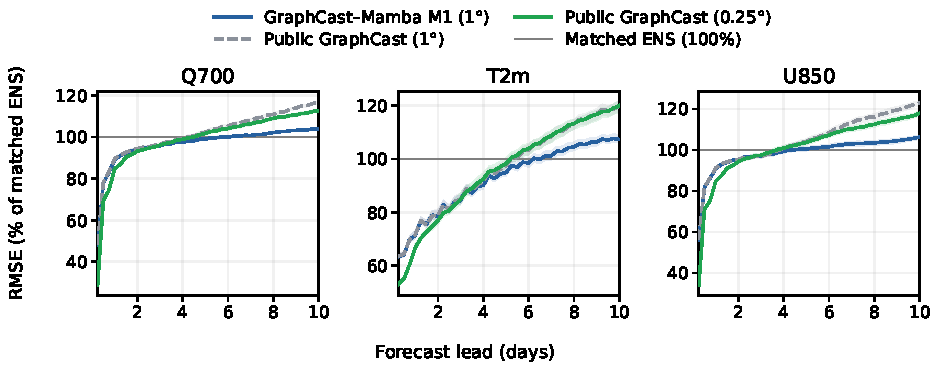
\includegraphics[width=\linewidth]{arxiv_pics/fig4_common_grid_comparison_v5_ci.pdf}
    \ifvfivechanges
\caption*{\color{vfiveDeleted}\sout{Comparison with higher-resolution GraphCast. From left to right: 700\,hPa specific humidity (Q700), $2$\,m temperature (T2m), and 850\,hPa zonal wind (U850). Blue shows the original selected GraphCast--Mamba model M1 at $1^\circ$, dashed gray its public GraphCast\_small baseline, and green the public GraphCast ($0.25^\circ$) reference. Forecasts are verified on a common $1.5^\circ$ grid; RMSE is expressed as a percentage of the ECMWF ensemble mean (ENS) reference, with $100\%$ indicating equal error. Each point uses identical ENS-available dates for all four forecasts (92--105 of 122 candidate starts in 2023). Squared errors are pooled before RMSE. Shading gives pointwise 95\% paired date-block-bootstrap intervals for fixed checkpoints, not seed variation (Appendix~\mbox{\ref{app:common_grid}}).}}
\fi
\caption{\vfiveadded{Comparison with higher-resolution GraphCast: \vfourchange{700\,hPa specific humidity (Q700)}, $2$\,m temperature (T2m), and 850\,hPa zonal wind (U850). Blue: \vfourchange{original M1} at $1^\circ$; dashed gray: \vfourchange{public GraphCast\_small}; green: \vfourchange{public} GraphCast ($0.25^\circ$). RMSE on the common $1.5^\circ$ grid is expressed relative to ENS \vfourchange{mean} ($100\%$). \vfourchange{All four forecasts use identical dates at each point (92--105 starts in 2023); squared errors are pooled before RMSE. Shading gives pointwise 95\% paired date-block-bootstrap intervals for fixed checkpoints, not seed variation (Appendix~\ref{app:common_grid}).}}}
    \label{fig:common_grid_selected}
\end{figure}

\subsection{Temporal memory contributes \vfourchange{to forecast skill}}
\label{sec:memory_ablation}
\ifvfivechanges
\par\begingroup\color{vfiveDeleted}\noindent
\sout{The preceding results show that GraphCast--Mamba improves forecasts at longer lead times across the predicted atmospheric state. The correction branch introduces both additional trainable capacity and temporal memory. To examine the contribution of temporal memory in the Mamba correction branch, we compare the selected model with a matched control trained and evaluated with memory reset at every step.}
\par\endgroup
\fi
\vfiveadded{The correction branch introduces both additional trainable capacity and temporal memory. To \vfourchange{examine} the contribution of memory, we \vfourchange{compare the selected model with a matched control trained and evaluated with memory reset at every step.}}

\ifvfivechanges
\par\begingroup\color{vfiveDeleted}\noindent
\sout{Table~\mbox{\ref{tab:memory_controls}} summarizes two policies obtained from two training runs in the original SWA comparison. The subsequent replication uses five carry-trained runs and one reset-trained run. Policy names specify memory handling during training first and forecasting second. Carry passes the updated SSM state and causal-convolution cache to the next step; reset zeros both before every step. Resetting leaves all learned weights and the two-frame meteorological input in place: the full correction branch still computes a correction, but cannot retain its temporal memory state between calls. Every training segment and independent forecast begins with a zero temporal memory state under both policies.}
\par\endgroup
\fi
\ifvfivechanges
\par\begingroup\color{vfiveDeleted}
\noindent\textit{Moved to Appendix A.2; original placement shown below.}\par
\begin{center}
    \centering
    \small
    \begin{tabular}{lcc}
        \toprule
\sout{Policy} & \multicolumn{2}{c}{\sout{Temporal memory retained}} \\
        \cmidrule(lr){2-3}
\sout{Training/forecasting} & \sout{Training} & \sout{Forecasting} \\
        \midrule
\sout{Carry/carry} & \sout{$\checkmark$} & \sout{$\checkmark$} \\
\sout{Reset/reset} & \sout{$\times$} & \sout{$\times$} \\
        \bottomrule
    \end{tabular}
    \captionof*{table}{\sout{Memory retained between successive steps: $\checkmark$ denotes retention; $\times$ denotes resetting both the SSM state and causal-convolution cache before every step. Reset/reset is trained separately with the same architecture and parameter count.}}
    
\end{center}
\par\endgroup
\fi
\vfiveadded{M1 retains the updated SSM states and causal-convolution caches during both training and forecasting. \ifvfivechanges{\color{vfiveDeleted}\sout{Its matched reset/reset control zeros both before every step}}\fi \vfiveadded{Its matched control, \textbf{R1}, resets both before every step during training and forecasting}, retaining all learned weights and the two-frame meteorological input. Every training segment and independent forecast begins with zero temporal memory under both policies. Table~\ref{tab:memory_controls} in Appendix~\ref{app:architecture_details} summarizes the policies. \vfourchange{The original SWA comparison uses one run per policy; the subsequent replication uses five retrainings of the M1 configuration and one reset-trained run.}}

The two training runs \vfourchange{in the original SWA comparison} use the same seven-year dataset, architecture, optimizer, and training seed, differing in their training/forecasting memory policy. Both use a training tail of $K=20$ feedback-conditioned steps, inner dimension $d_{\mathrm{inner}}=16$. \vfourchange{\vfiveRone{Reset/reset} is trained independently with memory reset in both its 500-update warm-up and 2,000-update main stage. Both configurations use the same batch size, optimizer schedule, and SWA checkpoint indices (Appendix~\ref{app:training_configuration}).} We evaluate \vfourchange{both} policies on the \vfourchange{same 122} forecast initializations and \vfourchange{40} lead times of Section~\ref{sec:eval_protocol}\vfourchange{, using a common GraphCast baseline}. Appendix~\ref{app:training_loss} describes the loss calculation for these controls\vfourchange{; Appendix~\ref{app:memory_evaluation} describes the paired uncertainty estimates}.

\begin{figure}[!htb]
    \centering
    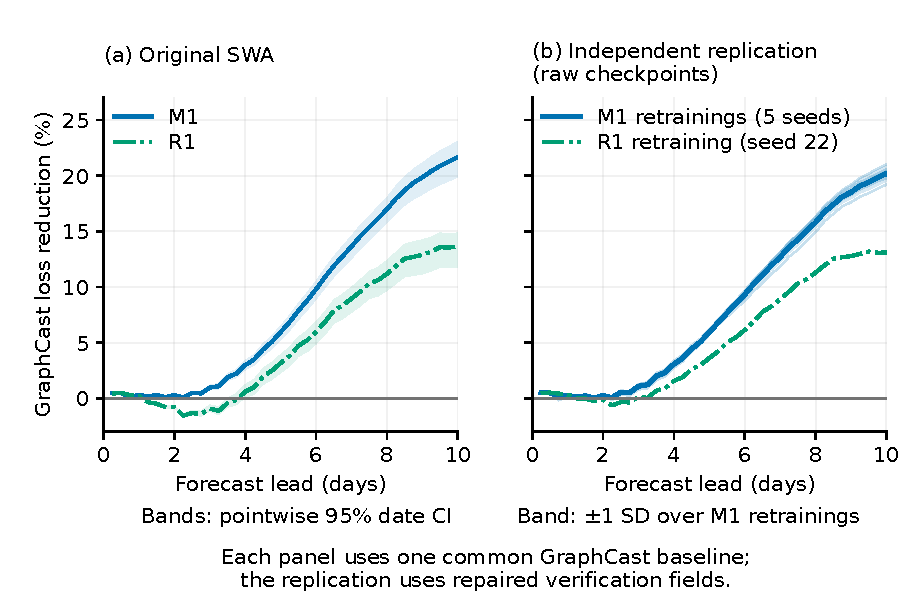
\includegraphics[width=0.8\linewidth]{arxiv_pics/fig5_memory_policies_v5_matched_only.pdf}
    \ifvfivechanges
\caption*{\color{vfiveDeleted}\sout{Comparison of carry/carry and reset/reset memory policies defined in Table~\mbox{\ref{tab:memory_controls}}. Curves show GraphCast loss reduction relative to a common public GraphCast baseline within each panel over ten forecast days. Left: original selected SWA checkpoint and matched SWA reset/reset control, with pointwise 95\% date-block-bootstrap intervals. Right: independent replication using raw main-step 2,000 checkpoints; five carry/carry seeds (thin curves, mean and one sample SD) versus the local seed-22 reset/reset control. The right-panel band describes carry/carry seed variation only; reset/reset has one training seed. SWA and raw checkpoints are not mixed within either comparison. Appendix~\mbox{\ref{app:seed_replication}} describes the replication.}}
\fi
\caption{\vfiveadded{\textbf{M1 and the \vfiveRone{reset/reset} control.} Curves show GraphCast loss reduction relative to \vfourchange{a common public GraphCast baseline within each panel}. \vfourchange{Left: M1 and matched SWA \vfiveRone{reset/reset} control, with pointwise 95\% date-block-bootstrap intervals. Right: raw main-step 2,000 checkpoints; five M1 retrainings (thin curves, mean and one sample SD) versus the local seed-22 \vfiveRone{reset/reset} \vfivewordchange{control}{retraining}. The right-panel band describes variation across M1 retrainings only; \vfivewordchange{reset/reset has one training seed}{the R1 configuration has one local training seed}. SWA and raw checkpoints are not mixed within either comparison (Appendix~\ref{app:seed_replication}).}}}
    \label{fig:memory_reset}
\end{figure}

\vfourchange{In the original matched SWA comparison, day-10 GraphCast loss reductions are $21.66\%$ for M1 and $13.64\%$ for \vfiveRone{reset/reset}. The M1 advantage is $8.02$ percentage points (pointwise 95\% confidence interval: $7.20$--$9.05$).}

\vfourchange{Over the full ten-day rollout, M1 achieves a $14.42\%$ GraphCast loss reduction, compared with $9.16\%$ for matched \vfiveRone{reset/reset}. The paired advantage is $5.26$ percentage points (pointwise 95\% confidence interval: $4.70$--$5.86$). Figure~\ref{fig:memory_reset} shows both policies. The matched training-policy comparison supports a benefit from persistent memory for this configuration and training realization. These intervals quantify forecast-sample uncertainty for fixed checkpoints, not variation across training seeds.}

\vfourchange{The independent raw-checkpoint replication in Figure~\ref{fig:memory_reset} yields reductions for the M1 configuration of $13.51\%\pm0.42$ percentage points over the rollout and $20.19\%\pm0.71$ percentage points at day 10 (five-seed mean $\pm$ SD). The local \vfiveRone{reset/reset} \vfivewordchange{control}{retraining} yields $9.21\%$ and $13.09\%$, respectively; all five M1 retrainings exceed this control at both endpoints. This adds replication of correction skill, but the single reset-trained seed does not establish the distribution of the memory-policy contrast across training seeds.}

\FloatBarrier
\subsection{\vfourred{Smoothing and spectral fidelity}}
\label{sec:smoothing}


\ifvfivechanges
\par\begingroup\color{vfiveDeleted}\noindent
\sout{It is known \mbox{\citep{lam2023graphcast,subich2025spectral}} that improvements in MSE can come at the cost of spatial detail: smoothing can reduce error while weakening small-scale structures. In order to investigate these effects we also examine spatial power spectra of forecast by assessing whether predictions preserve variability across spatial scales.  In particular, we compare the learned correction with an optimally smoothing filter applying to the GraphCast baseline to assess whether similar accuracy gains can be obtained through output smoothing and how the two approaches differ in spectral fidelity.}
\par\endgroup
\fi
\vfiveadded{\vfourred{Improvements in MSE can come at the cost of spatial detail: smoothing can reduce error while weakening small-scale structures~\citep{lam2023graphcast,subich2025spectral}. We therefore examine forecast power spectra and compare the learned correction with an optimally fitted GraphCast output filter, assessing whether smoothing reproduces its accuracy and spectral fidelity.}}

% Prior spectral draft wording, retained internally:
% \vfourred{Following the filter construction in \citet[Supplementary Section~7.4.2]{lam2023graphcast}, we transform GraphCast forecasts into spherical harmonics and fit one multiplicative gain per forecast lead, variable/pressure level and total wavenumber. The gains minimize coefficient-domain squared error on 32 development initializations from 2022. We freeze them before evaluation and filter only the reported outputs, leaving autoregressive feedback unchanged. ``Optimal'' refers to this fitted linear filter family. We compare raw GraphCast, GraphCast plus the optimal filter, M1 and matched reset/reset on the same fixed 36 initializations from January--April 2023. Both correction models retain their original unfiltered outputs.}
\begin{figure}[!t]
    \centering
% Before the variable-spectrum revision:
%     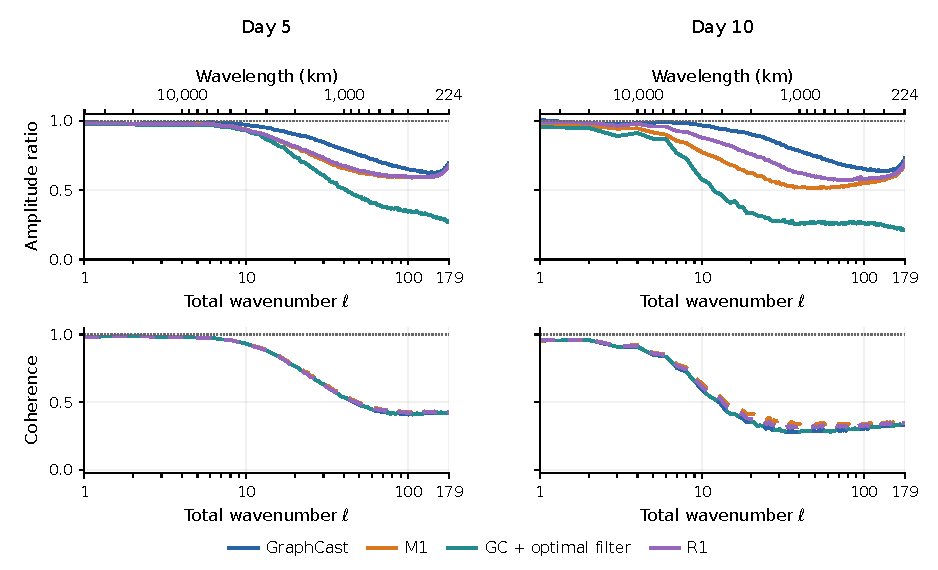
\includegraphics[width=\linewidth]{arxiv_pics/fig6_smoothing_day5_day10_v5_matched122.pdf}
    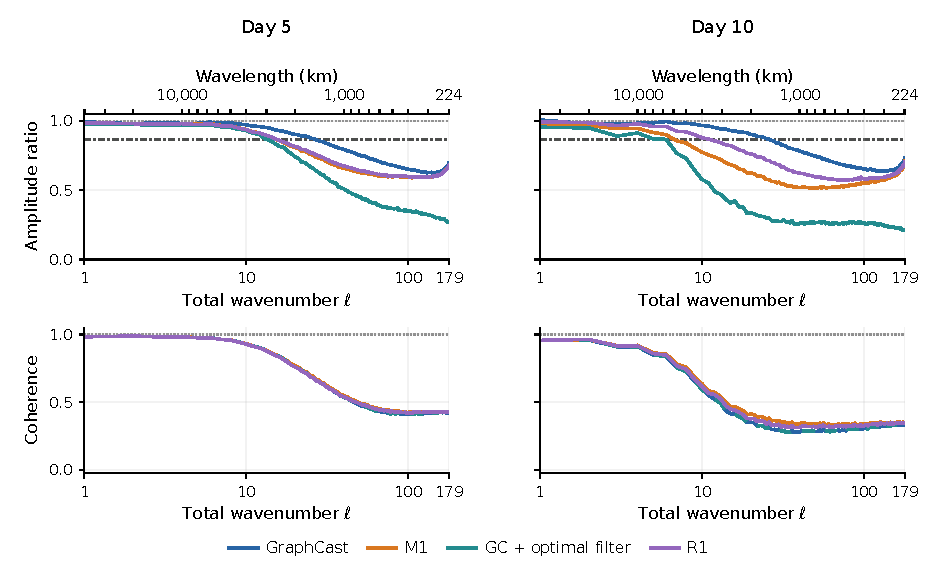
\includegraphics[width=\linewidth]{arxiv_pics/fig6_smoothing_day5_day10_v5_variables122.pdf}
% Before clarifying the attenuation reference:
%     \caption{\vfourred{Amplitude ratio (top) and coherence (bottom) at day 5 (left) and day 10 (right) on the 122 evaluation initializations. Channel-wise ratios are formed after pooling dates and averaged across all 83 channels with GraphCast variable/pressure weights. An amplitude ratio of one denotes power matching. The $\sqrt{0.75}$ line is a weighted-amplitude reference, not a threshold on mean power loss. Positive filter gains preserve GraphCast coherence; complementary dashes retain both curves. Appendix~\ref{app:smoothing} gives definitions and per-variable diagnostics.}}
    \caption{\vfourred{Amplitude ratio (top) and coherence (bottom) at day 5 (left) and day 10 (right) on the 122 evaluation initializations. Curves average date-pooled channel ratios across all 83 channels with GraphCast variable/pressure weights. The dash-dotted line at $\sqrt{0.75}\simeq0.866$ follows the attenuation reference of \citet{subich2025spectral}: for an individual channel, it corresponds to retaining 75\% of ERA5 power at that scale. Its first downward crossing compares where this level of attenuation is reached; crossing at a lower wavenumber means coarser scales are affected. The text explains its use for averaged amplitudes. Positive filter gains preserve GraphCast coherence; complementary dashes retain both curves.}}
% Prior spectral draft wording, retained internally:
%     \caption{\vfourred{Amplitude ratio (top) and coherence (bottom) at day 5 (left) and day 10 (right) for the four predictors on the fixed 36-date cohort. An amplitude ratio of one denotes power matching; coherence measures normalized cross-power. Channel-wise ratios are formed after pooling dates and averaged with GraphCast variable/pressure weights. Positive output-filter gains preserve GraphCast coherence; complementary dashes retain both curves. Appendix~\ref{app:smoothing} gives the definitions and the effect of negative gains.}}
% Before the variable-spectrum revision:
%     \caption{\vfourred{Amplitude ratio (top) and coherence (bottom) at day 5 (left) and day 10 (right) for the four predictors on the 122 evaluation initializations. An amplitude ratio of one denotes power matching; coherence measures normalized cross-power. Channel-wise ratios are formed after pooling dates and averaged with GraphCast variable/pressure weights. Positive output-filter gains preserve GraphCast coherence; complementary dashes retain both curves. Appendix~\ref{app:smoothing} gives the definitions and the effect of negative gains.}}
    \label{fig:smoothing_spectra}
\end{figure}

\vfourred{Following the filter construction in \citet[Supplementary Section~7.4.2]{lam2023graphcast}, we transform GraphCast forecasts into spherical harmonics and fit one multiplicative gain per forecast lead, variable/pressure level and total wavenumber. The gains minimize coefficient-domain squared error on 32 development initializations from 2022. We freeze them before evaluation and filter only the reported outputs, leaving autoregressive feedback unchanged. ``Optimal'' refers to this fitted linear filter family. The comparison of raw GraphCast, GraphCast plus the optimal filter, M1 and matched \vfiveRone{reset/reset} uses the same 122 initializations and 40 six-hour leads as Section~\ref{sec:eval_protocol}. Both correction models retain their original unfiltered outputs.}

% Interim-only review material archived internally; not rendered.
% \ifvfivechanges
% \par\begingroup\color{vfiveDeleted}\noindent
% \sout{Figure~\mbox{\ref{fig:smoothing_spectra}} shows the spectral amplitude ratio (the square root of forecast-to-ERA5 power) and coherence at days 5 and 10. Coherence measures pattern agreement separately from amplitude \mbox{\citep{subich2025spectral}}. Table~\mbox{\ref{tab:smoothing_scores}} reports percentage reductions in exact GraphCast-weighted MSE and aggregate power mismatch relative to raw GraphCast over the rollout and at days 5 and 10. Power mismatch averages the absolute relative departure from ERA5 power across channels and wavenumbers; Appendix~\mbox{\ref{app:smoothing}} defines the metrics and provides the filtering equations, per-variable spectra and numerical details. These fixed-checkpoint diagnostics are separate from the principal 122-date memory comparison.}
% \par\endgroup
% \fi
% Prior spectral draft wording, retained internally:
% \vfiveadded{\vfourred{Figure~\ref{fig:smoothing_spectra} shows the spectral amplitude ratio (the square root of forecast-to-ERA5 power) and coherence at days 5 and 10. Coherence measures pattern agreement separately from amplitude \citep{subich2025spectral}. Table~\ref{tab:smoothing_scores} reports exact GraphCast-weighted MSE and aggregate power mismatch as ratios to raw GraphCast over the rollout and at days 5 and 10. Power mismatch averages the absolute relative departure from ERA5 power across channels and wavenumbers; Appendix~\ref{app:smoothing} defines the metrics and provides the filtering equations, per-variable spectra and numerical details. These fixed-checkpoint diagnostics are separate from the principal 122-date memory comparison.}}
% Before the variable-spectrum revision:
% \vfiveadded{\vfourred{Figure~\ref{fig:smoothing_spectra} shows the spectral amplitude ratio (the square root of forecast-to-ERA5 power) and coherence at days 5 and 10. Coherence measures pattern agreement separately from amplitude \citep{subich2025spectral}. Table~\ref{tab:smoothing_scores} reports exact GraphCast-weighted MSE and aggregate power mismatch as ratios to raw GraphCast over the rollout and at days 5 and 10. Power mismatch averages the absolute relative departure from ERA5 power across channels and wavenumbers; Appendix~\ref{app:smoothing} defines the metrics and provides the filtering equations, per-variable spectra and numerical details.}}
% Before clarifying the attenuation reference:
% \vfourchange{\vfourred{Figure~\ref{fig:smoothing_spectra} compares spectral amplitude ratios (the square root of forecast-to-ERA5 power) and coherence, which measures pattern agreement separately from amplitude~\citep{subich2025spectral}. Appendix~\ref{app:smoothing} pairs day-5 and day-10 spectra for four illustrative fields with their native-grid RMSE reductions. Table~\ref{tab:smoothing_scores} there retains the aggregate comparison: exact GraphCast-weighted MSE and power mismatch, the latter averaging absolute relative power departures equally across channels and wavenumbers.}}
\vfourchange{\vfourred{Following \citet[Section~3.1]{subich2025spectral}, Figure~\ref{fig:smoothing_spectra} compares amplitude ratios (the square root of forecast-to-ERA5 power) and coherence, separating attenuation from spatial-pattern agreement. We also adopt their illustrative amplitude reference $\sqrt{0.75}\simeq0.866$, corresponding to a 25\% power deficit for an individual channel and scale. A first crossing at a lower wavenumber indicates attenuation reaching coarser scales; falling farther below the line indicates stronger attenuation. Here the curves average channel-wise amplitude ratios, so their crossings compare mean attenuation rather than locating an exact 25\% deficit in averaged power. Appendix~\ref{app:smoothing} pairs per-variable spectra with native-grid RMSE; Table~\ref{tab:smoothing_scores} retains the aggregate MSE and equal-degree power-mismatch comparison.}}

\ifvfivechanges
\par\noindent\textit{V5 layout change: removed the forced float barrier here.}\par
\fi


% Before the variable-spectrum revision:
% \vfourred{The day-5 comparison supports the proposed architecture: M1 has $2.85\%$ lower MSE than \vfiveRone{reset/reset}, with $0.50$ percentage points higher aggregate power mismatch ($69.60\%$ versus $69.10\%$). It also improves on filtered GraphCast in both MSE and power mismatch. Over the full rollout, M1 retains $4.02\%$ lower MSE than filtered GraphCast, with power mismatch $67.56\%$ versus $78.40\%$. Thus the tested output filter does not reproduce the correction's accuracy--spectral-fidelity performance. Raw GraphCast retains closer aggregate power matching than either correction model.}
% Before clarifying the attenuation reference:
% \vfiveadded{At day 5, M1 has $2.85\%$ lower MSE than \vfourchange{R1}, with similar aggregate power mismatch ($69.60\%$ versus $69.10\%$, a difference of $0.50$ percentage points). Over the full rollout, M1 also has $4.02\%$ lower MSE than filtered GraphCast and lower power mismatch ($67.56\%$ versus $78.40\%$). Thus the tested output filter does not reproduce M1's joint accuracy and spectral-fidelity performance. Raw GraphCast already has substantial mismatch under this metric ($59.47\%$ over the rollout), but retains closer aggregate power matching than either correction model.}
\vfiveadded{At day 5, M1 and \vfourchange{R1} have closely overlapping amplitude and coherence curves, and both amplitude curves first fall below the reference at sampled wavenumber $\ell=16$. M1 achieves $2.85\%$ lower MSE with similar aggregate power mismatch ($69.60\%$ versus $69.10\%$, a difference of $0.50$ percentage points). Over the full rollout, M1 also has $4.02\%$ lower MSE than filtered GraphCast and lower power mismatch ($67.56\%$ versus $78.40\%$). Thus the tested output filter does not reproduce M1's joint accuracy and spectral-fidelity performance. Raw GraphCast already has substantial mismatch under this metric ($59.47\%$ over the rollout), but retains closer aggregate power matching than either correction model.}

% Before the variable-spectrum revision:
% \vfourred{By day 10, all four forecasts have substantially larger absolute errors and reduced spectral coherence compared with day 5 (Figure~\ref{fig:smoothing_spectra}; Appendix~\ref{app:smoothing_features}); M1's MSE, for example, rises from $7.83$ to $23.30$. Its $9.26\%$ MSE advantage over \vfiveRone{reset/reset} at day 10 accompanies a larger power-mismatch difference ($84.34\%$ versus $76.38\%$). This longer lead extends beyond the five-day feedback-conditioned training tail. The day-5 result therefore provides the clearest support for an accuracy gain with a small aggregate spectral cost; the day-10 results document a more degraded forecasting regime and do not establish a uniformly better tradeoff than \vfiveRone{reset/reset}.}
% Before clarifying the attenuation reference:
% \vfiveadded{At day 10, beyond the five-day feedback-conditioned training tail, M1's $9.26\%$ MSE advantage over \vfourchange{R1} accompanies stronger attenuation over much of the spectrum and a larger aggregate power mismatch ($84.34\%$ versus $76.38\%$). The per-variable results distinguish retained structure, accuracy--attenuation tradeoffs, and an adverse humidity example (Appendix~\ref{app:smoothing_features}). These fixed-checkpoint results support a memory benefit in accuracy with similar aggregate mismatch at day 5; they do not establish uniform improvement across variables, scales, or leads.}
\vfiveadded{At day 10, beyond the five-day feedback-conditioned training tail, the first reference crossings separate to $\ell=7$ for M1 and $\ell=12$ for \vfourchange{R1}. M1's $9.26\%$ MSE advantage accompanies stronger attenuation over much of the spectrum, despite generally slightly higher coherence, and larger aggregate power mismatch ($84.34\%$ versus $76.38\%$). The per-variable results further resolve these tradeoffs (Appendix~\ref{app:smoothing_features}). These fixed-checkpoint results support a memory benefit in accuracy with similar combined spectral behavior at day 5; they do not establish uniform improvement across variables, scales, or leads.}

% Interim-only review material archived internally; not rendered.
% \ifvfivechanges
% \par\begingroup\color{vfiveDeleted}
% \noindent\textit{Previous table: loss reductions (replaced by relative errors below).}\par
% \begin{center}
%     \centering
%     \begingroup\small
%     \setlength{\tabcolsep}{4pt}
%     \begin{tabular}{lrrrrrr}
%         \toprule
% \multicolumn{7}{c}{\sout{Reduction relative to raw GraphCast (\%) $\uparrow$}} \\
%         \addlinespace[2pt]
%  & \multicolumn{2}{c}{\sout{Ten-day rollout}} & \multicolumn{2}{c}{\sout{Day 5}} & \multicolumn{2}{c}{\sout{Day 10}} \\
%         \cmidrule(lr){2-3}\cmidrule(lr){4-5}\cmidrule(lr){6-7}
% \sout{Forecast} & \shortstack{\sout{MSE}\\\sout{reduction}} & \shortstack{\sout{Power}\\\sout{mismatch}\\\sout{reduction}} & \shortstack{\sout{MSE}\\\sout{reduction}} & \shortstack{\sout{Power}\\\sout{mismatch}\\\sout{reduction}} & \shortstack{\sout{MSE}\\\sout{reduction}} & \shortstack{\sout{Power}\\\sout{mismatch}\\\sout{reduction}} \\
%         \midrule
% \sout{Raw GraphCast} & \sout{0.00} & \sout{0.00} & \sout{0.00} & \sout{0.00} & \sout{0.00} & \sout{0.00} \\
% \sout{GraphCast + optimal filter} & \sout{11.34} & \sout{$-33.60$} & \sout{4.16} & \sout{$-36.09$} & \sout{18.98} & \sout{$-42.35$} \\
% \sout{Carry/carry (M1)} & \sout{15.10} & \sout{$-14.59$} & \sout{6.05} & \sout{$-13.65$} & \sout{23.42} & \sout{$-30.61$} \\
% \sout{Reset/reset} & \sout{9.67} & \sout{$-11.65$} & \sout{3.30} & \sout{$-12.83$} & \sout{14.72} & \sout{$-17.11$} \\
%         \bottomrule
%     \end{tabular}
%     \endgroup
%     \captionof*{table}{\sout{Percentage reductions relative to raw GraphCast on the fixed 36-date cohort: $100(1-L/L_{\mathrm{GC}})$ for exact GraphCast MSE and $100(1-D_P/D_{P,\mathrm{GC}})$ for aggregate power mismatch. Rollout scores pool all forty leads. Positive values indicate improvement; negative values indicate deterioration. Zero denotes baseline performance, not zero error. The metrics measure distinct quantities; both correction models are unfiltered. Appendix~\mbox{\ref{app:smoothing}} defines $D_P$ and the evaluation procedure. Values are fixed-checkpoint point estimates.}}
%
% \end{center}
% \par\endgroup
% \fi
% Aggregate comparison table moved to Appendix C.


\section{Conclusion}

Our results show that a small correction branch with persistent temporal memory can improve forecasts from a frozen pretrained weather model at longer forecast lead times. \vfourchange{Five independent retrainings reproduce the correction benefit. The matched reset-trained control supports a memory benefit for the tested configuration and training realization.} This suggests that compact temporal extensions offer a promising way to improve existing forecasters with limited additional training. How this benefit depends on spatial resolution and the choice of backbone remains an open question.

\vfourchange{{\textbf{Limitations.} Our results show that non-Markovian memory can improve forecasts from a frozen Markovian backbone. This suggests the possibility of jointly learning the forecasting dynamics and temporal memory within a native model. However, autoregressive training introduces sequential dependencies between forecast steps, limiting temporal parallelism and opportunities for batching and data reuse. Backpropagation through long rollouts also requires storing or recomputing intermediate activations, making efficient computation and memory access central challenges for joint training of the full model. To keep training tractable, our study restricts learning to a correction branch attached to a frozen pretrained forecaster.

\vfourred{Lower aggregate forecast error does not by itself establish recovery of fine-scale variability. Section~\ref{sec:smoothing} and Appendix~\ref{app:smoothing} examine the associated power-spectrum changes and the scope of the filtering and memory comparisons.}}}
\FloatBarrier


% ICLR 2027 requires an AI use statement, excluded from the page limit.
% AUTHOR TODO: Add a statement reflecting the full study-wide history and the
% authors' verification. Template migration and manuscript review used AI.
% V3 AUTHOR TODO: Verify the statement below against the full study-wide history
% and document the authors' checks before submission.
% Keep this as an author action rather than inserting unapproved manuscript prose.
% V4 SEED UPDATE TODO: The assistant implemented bootstrap analysis and figures;
% the inherited no-analysis-assistance claim below must be reviewed by authors.
\clearpage
\section*{AI use statement}

We used a large language model for minor editorial assistance, including correcting grammar and
typo and refining formatting. It did not contribute to the development of research ideas, the analysis,
or the claims.

\section*{Ethics Statement}
All datasets, models in this work are publicly available. The usage of these datasets, models, code strictly follows the terms and conditions set by the providers. 

\section*{Reproducibility Statement}
To ensure reproducibility of our results, we provide detailed documentation of our experimental setup and methodology in the main paper and appendix. The code for data, evaluation,
and training will be open-sourced upon publication.


% suozhi 原话：我们最后需要 AI statement。
% \suozhi{We need to include an AI use statement before submitting the paper.}

\bibliographystyle{iclr2027_conference}
\bibliography{bib,arxiv_references}

\clearpage
\appendix

\section{\texorpdfstring{\vfourchange{Training and supporting evaluations}}{Training and supporting evaluations}}
\label{app:training}

\vfourchange{This appendix gives the training configuration for M1 and \vfivewordchange{its reset control}{R1}, followed by the architecture and loss definitions. It then describes the memory-control evaluation and five-seed replication (Sections~\ref{app:memory_evaluation}--\ref{app:seed_replication}), the development-set studies used for model selection, and the variable-group errors and computational costs supporting the main results.}

\subsection{Training configuration}
\label{app:training_configuration}

\paragraph{\vfourchange{Data preparation.}}
\vfourchange{We use six-hourly ERA5 data from WeatherBench 2, subsampled to $1^\circ$ by selecting every fourth grid point in each spatial dimension, with GraphCast's 13 pressure levels and supplied normalization statistics.}

\paragraph{\vfourchange{Initialization and batching.}}
\vfourchange{The correction branch copies the pretrained GraphCast encoder, decoder, and first two graph message-passing steps, inserts newly initialized Mamba modules, and uses a zero-initialized output head. We train all correction parameters while keeping the backbone frozen. Each update processes one 24-step window from each of four independent segments ($B=4$), using the memory and feedback procedure in Section~\ref{sec:training}.}

\paragraph{\vfourchange{Optimization and checkpoint averaging.}}
\vfourchange{Training comprises a 500-update initialization stage, called warm-up in the main text, followed by 2,000 updates that transfer the learned weights to a fresh optimizer. Both stages linearly increase the spatial learning rate from zero to $10^{-4}$ over 50 updates. The first stage then holds this rate constant and uses the same rate for Mamba parameters. The second applies cosine decay toward $10^{-5}$ over the remaining 1,950 updates, with Mamba's rate three times the spatial rate throughout.}

\vfourchange{Both stages use AdamW with moments $(0.9,0.98)$, weight decay $10^{-4}$ on all trainable correction parameters, and global gradient-norm clipping at 1. M1 uses seed 22 and bfloat16 computation, with float32 meteorological fields and temporal-state boundaries. Evaluation uses SWA over second-stage updates 500, 1,000, 1,500, and 2,000.}
% Operational detail: the main stage restarts the random-number generator,
% temporal memory, and data cursor as well as the optimizer.

\paragraph{\vfourchange{Matched reset control.}}
\vfourchange{The \vfiveRone{reset/reset} control matches M1's architecture, parameter count, data, batch size, seed, precision, optimizer schedule, and SWA indices. It resets both SSM states and convolution caches before every prediction during training and forecasting, and starts its main stage from its own reset-trained initialization weights. The 24-step windows, $K=20$ feedback-conditioned tail, full correction feedback, and loss are unchanged. Hyperparameters are fixed without further model selection. The control matches M1's configured protocol; its software environment was reconstructed.}
% Provenance: the control uses recovered archived training and model code;
% previously unarchived dependencies were supplied from the workspace and
% frozen for the new run. The incomplete historical environment prevents a
% claim of bitwise reproduction of the earlier run.

\ifvfivechanges
\par\noindent\textit{Previous training description (replaced above).}\par
\fi
\ifvfivechanges
\par\begingroup\color{vfiveDeleted}\noindent
\sout{Training examples are drawn from ERA5 2015--2021, with 2022 reserved for development. These data come from the six-hourly WeatherBench2 ERA5 archive,}\footnote{\path{gs://weatherbench2/datasets/era5/1959-2023_01_10-wb13-6h-1440x721_with_derived_variables.zarr}.}\sout{ subsampled by selecting every fourth latitude and longitude of the $0.25^\circ$ grid to obtain a $181\times360$ grid at $1^\circ$. We retain pressure levels 50, 100, 150, 200, 250, 300, 400, 500, 600, 700, 850, 925, and 1000\,hPa. We reuse the GraphCast normalization files \path{mean_by_level.nc}, \path{stddev_by_level.nc}, and \path{diffs_stddev_by_level.nc}, distributed under \path{gs://dm_graphcast/graphcast/stats/}, throughout correction training and evaluation.}
\par\endgroup
\fi

\ifvfivechanges
\par\begingroup\color{vfiveDeleted}\noindent
\sout{We initialize the Mamba correction branch from the frozen GraphCast backbone checkpoint: its grid-to-mesh encoder (G2M), mesh-to-grid decoder (M2G), and two graph message-passing steps copy the corresponding pretrained weights, using the first two of GraphCast's 16 graph message-passing steps. We insert newly initialized Mamba modules after these graph message-passing steps and append a linear output head with weights and biases initialized to zero. Consequently, the initial forecast correction is zero and the GraphCast--Mamba forecast equals the pretrained GraphCast backbone forecast. The copied spatial parameters, Mamba modules, and output head form the trainable parameters $\phi$; the separate GraphCast backbone parameters $\theta$ remain frozen throughout training on ERA5 2015--2021. Each optimizer update processes one window from each of four independent segments, giving batch size $B=4$ under the memory-carry procedure in Section~\mbox{\ref{sec:training}}.}
\par\endgroup
\fi

\ifvfivechanges
\par\begingroup\color{vfiveDeleted}\noindent
\sout{The reported model uses two optimization stages. The first stage, called the 500-update warm-up in the main text, linearly increases the learning rate from zero to $10^{-4}$ over its first 50 updates and then holds it constant. Spatial and Mamba parameters use the same learning rate during this stage. The second stage transfers the learned correction weights and starts a fresh optimizer for 2,000 further updates, resetting the random-number generator, temporal memory, and data cursor. Its spatial learning rate ramps from zero to $10^{-4}$ over 50 updates and then follows cosine decay toward $10^{-5}$ over the remaining 1,950 updates. The Mamba learning rate is three times the spatial learning rate throughout this second stage.}
\par\endgroup
\fi

\ifvfivechanges
\par\begingroup\color{vfiveDeleted}\noindent
\sout{Both stages use AdamW with moments $(0.9,0.98)$, weight decay $10^{-4}$ applied to all trainable correction parameters, global gradient-norm clipping at 1, and random seed 22. Model computation uses bfloat16, with float32 meteorological fields and temporal-state boundaries. The configuration uses spatial width 512, inner dimension 16, and one $B,C$ group. The evaluated model averages the parameters saved at second-stage updates 500, 1,000, 1,500, and 2,000 using SWA; these are the post-warm-up checkpoint indices used elsewhere in the paper.}
\par\endgroup
\fi

\ifvfivechanges
\par\begingroup\color{vfiveDeleted}\noindent
\sout{The reset/reset control uses the same backbone, training data, correction architecture, parameter count, batch size four, random seed 22, precision, optimizer schedules, and SWA indices as the selected carry-trained model. Both its 500-update warm-up and 2,000-update main stage reset the SSM states and causal-convolution caches before every correction prediction; the main stage starts from its own reset-trained warm-up weights. The 24-step training windows, $K=20$ feedback-conditioned tail, full correction feedback, and loss objective are retained. Hyperparameters are fixed to the selected configuration without further model selection. The control uses the recovered archived training and model code, with previously unarchived dependencies supplied from the workspace and frozen for the new run. The historical environment was not fully archived, so matching refers to the configured training protocol and does not imply bitwise reproduction of the earlier run.}
\par\endgroup
\fi

\subsection{Architecture and memory implementation}
\label{app:architecture_details}
% V5: detailed notation, training schematic, and policy table retained from v4.
\paragraph{Graph representation.}
\vfiveadded{The GraphCast backbone operates on a latitude--longitude grid and an auxiliary mesh, with graph $\mathcal{G}(\mathcal{V}^{\textrm{G}},\mathcal{V}^{\textrm{M}},\mathcal{E}^{\textrm{G2M}},\mathcal{E}^{\textrm{M}},\mathcal{E}^{\textrm{M2G}})$. The vertices $\mathcal{V}^{\textrm{G}}$ represent the meteorological grid and $\mathcal{V}^{\textrm{M}}$ the mesh. Encoding uses grid-to-mesh edges $\mathcal{E}^{\textrm{G2M}}$, followed by $N=16$ graph message-passing steps over $\mathcal{E}^{\textrm{M}}$ and decoding over mesh-to-grid edges $\mathcal{E}^{\textrm{M2G}}$. Latent node features have width $W_{\textrm{GC}}=512$.}

\paragraph{Mamba dimensions and correction path.}
\vfiveadded{Our model uses an SSM state dimension of $16$ per inner channel, a causal convolution width of $4$, a rank-$32$ projection for the step-size parameter $\Delta_t$, and one shared group of input-dependent $B_t,C_t$ coefficients. Additional studies examine $d_{\mathrm{inner}}=32$. The memory-reset controls in Section~\ref{sec:memory_ablation} use $d_{\mathrm{inner}}=16$ and one shared $B,C$ group.}
\vfiveadded{Suppressing the direct encoder-to-decoder grid-feature connection, the correction branch's mesh-processing path is}
\begin{align}
    L_t^{(0)} &= \operatorname{Encode}_\phi(X_t),\\
    \widetilde{L}_t^{(k)} &= \operatorname{GNN}^{(k)}_\phi(L_t^{(k-1)}),\\
    (L_t^{(k)},m_t^{(k)})
    &=\operatorname{MambaModule}^{(k)}_\phi
       (\widetilde{L}_t^{(k)},m_{t-1}^{(k)}),\qquad k=1,2,\\
    c_t &= \operatorname{Decode}_\phi(L_t^{(2)}).
\end{align}
\vfiveadded{Each Mamba module contains two residual Mamba layers; $m_t^{(k)}$ comprises their SSM states and causal-convolution caches.}

\begin{figure}[!htbp]
    \centering
    \normalsize
    \[
    m_{\mathrm{init}}=0\;\longrightarrow\;
    \underbrace{
      \boxed{1{:}24}
      \xrightarrow{\mathrm{sg}}\boxed{25{:}48}
      \xrightarrow{\mathrm{sg}}\boxed{49{:}72}
      \xrightarrow{\mathrm{sg}}\boxed{73{:}96}
    }_{\text{one segment: memory carried through 96 steps}}
    \xrightarrow{\mathrm{reset}}\;m_{\mathrm{init}}'=0
    \]
    \caption{Memory carry during training. Boxes show the four 24-step windows of one segment. The arrows marked $\mathrm{sg}$ carry the SSM states and causal-convolution caches unchanged across window boundaries while stopping their gradients. Both are reset for the next segment.}
    \label{fig:training_segments}
\end{figure}

\begin{table}[!htb]
    \centering
    \small
    \begin{tabular}{lcc}
        \toprule
        \vfourchange{Model} & \multicolumn{2}{c}{Temporal memory retained} \\
        \cmidrule(lr){2-3}
        & Training & Forecasting \\
        \midrule
        \vfourchange{M1} & $\checkmark$ & $\checkmark$ \\
        \vfiveRone{Reset/reset} & $\times$ & $\times$ \\
        \bottomrule
    \end{tabular}
    \caption{Memory retained between successive steps: $\checkmark$ denotes retention; $\times$ denotes resetting both the SSM state and causal-convolution cache before every step. \vfiveRone{Reset/reset} is trained separately with the same architecture and parameter count.}
    \label{tab:memory_controls}
\end{table}

\subsection{Complete loss definition}
\label{app:training_loss}
The per-step loss in Equation~\ref{eq:training_objective} is the {GraphCast loss}:
\begin{equation}
    \ell_{\mathrm{GC}}(\hat{Y},Y)
    =\sum_v\frac{\lambda_v}{N_{\mathrm{g}}L_v}
      \sum_{i=1}^{N_{\mathrm{g}}}\sum_{\ell=1}^{L_v}
      a_i q_{v,\ell}
      \left(\frac{\hat{Y}_{v,\ell,i}-Y_{v,\ell,i}}
      {\sigma_{v,\ell}}\right)^2.
    \label{eq:training_gc_loss}
\end{equation}
Here $N_{\mathrm{g}}$ is the number of grid points and $L_v$ is the number of levels for variable $v$. The scales $\sigma_{v,\ell}$ are GraphCast's standard deviations of six-hour differences. The latitude weights $a_i$ have unit mean and include the pole-cell correction. For upper-air variables, $q_{v,\ell}=p_\ell/\overline{p}$ weights levels in proportion to pressure; surface variables have $L_v=1$ and $q_{v,1}=1$. The variable weights $\lambda_v$ are 1 for upper-air variables and $2$\,m temperature, and 0.1 for the two $10$\,m wind components, mean sea-level pressure, and six-hour accumulated precipitation.

\paragraph{{Evaluation variants.}}
We use GraphCast loss as the common label for the weighted MSE diagnostics. The principal results \vfourchange{and updated 2023 memory comparisons} evaluate Equation~\ref{eq:training_gc_loss} directly. \vfourchange{Memory-policy comparisons use a common GraphCast baseline within each comparison, whereas Figure~\ref{fig:res1_forecast} uses each seed's paired baseline.} The closed-loop training-tail sweep \vfourchange{reconstructs} it from channel RMSEs using per-level normalization and pressure weights, without the pole-cell correction. The archived open-loop sweep instead uses variable-group RMSEs and level-averaged normalization scales. These reconstructions therefore approximate the loss above.

\subsection{\vfourchange{Memory-control evaluation and uncertainty}}
\label{app:memory_evaluation}

\vfourchange{The original matched SWA comparison reuses the original frozen evaluator, initialization manifest, input data, and normalization statistics. M1 reuses its original forecast files. Both policies start with zero temporal memory, feed back their full corrected forecasts, and are scored on the same 122 initializations and 40 six-hour leads; late-December forecasts use verifying ERA5 states through 9 January 2024. All loss reductions in this comparison use the original M1 evaluation's uncorrected GraphCast trajectory as their common denominator, pooling losses before computing ratios. The independent raw-checkpoint replication is specified separately below.}

\ifvfivechanges
\par\begingroup\color{vfiveDeleted}\noindent
\sout{The M1 versus matched reset/reset rollout contrast is a separate planned analysis added after the original selected-model evaluation; it is not part of that evaluation's original confirmatory endpoint family. Day 10 is a secondary endpoint. We resample complete paired forecasts using 10,000 non-wrapping block-bootstrap draws with seed 20260916 and blocks of five consecutive initialization positions (12 elapsed days). Intervals for reductions, contrasts, and leadwise curves are pointwise 95\% intervals, conditional on the fixed checkpoints and the 2023 sample. They do not measure training-seed or between-year variation, or establish simultaneous significance across leads.}
\par\endgroup
\fi
\vfourchange{The M1 versus \vfiveRone{reset/reset} rollout contrast was planned after the original selected-model evaluation, outside its confirmatory endpoint family; day 10 is secondary. We use 10,000 paired, non-wrapping block-bootstrap draws (seed 20260916), with blocks of five consecutive positions on the regular 122-date grid (12 elapsed days). Each draw concatenates sampled blocks and truncates to 122 positions. Losses are pooled within each draw before forming ratios or contrasts; the 2.5th and 97.5th percentiles give pointwise 95\% intervals. These intervals concern the fixed checkpoints and 2023 sample, not training-seed or between-year variation or simultaneous significance across leads.}

\vfourchange{The positive rollout contrast persists with three-start and seven-start blocks and with resampling within calendar quarters. These checks do not remove dependence from overlapping forecast windows. Non-wrapping blocks underweight boundary dates, and quarter-wise resampling breaks dependence across quarter boundaries.}

\vfourchange{Repeated uncorrected GraphCast evaluations differ numerically. For \vfiveRone{reset/reset}, the pooled baseline loss differs by $0.0872\%$ from the common baseline, with a largest initialization/lead difference of $4.39\%$. Using each policy's own repeated baseline instead gives an M1 versus \vfiveRone{reset/reset} rollout contrast of $5.34$ percentage points (95\% interval: $4.78$--$5.95$), preserving the conclusion. The reported main estimates consistently use the common baseline.}



\subsection{\vfourchange{Five-seed replication and uncertainty scope}}
\label{app:seed_replication}

\ifvfivechanges
\par\begingroup\color{vfiveDeleted}\noindent
\sout{We evaluate five fresh retrainings of the M1 configuration with seeds 22--26, each with its own 500-update warm-up and 2,000-update main stage. They hold fixed the selected training data (2015--2021), $K=20$, batch size four, $d_{\mathrm{inner}}=16$, architecture, loss, optimizer and learning-rate schedules in Appendix~\mbox{\ref{app:training_configuration}}. Each SWA averages main-stage checkpoints 500, 1,000, 1,500 and 2,000. The recipe was reconstructed from the paper and repository configurations because the original training configurations and frozen environment were unavailable for this replication. Local seed 22 is a fresh retraining, not the historical selected checkpoint; the latter is not included in the five-seed mean. The configuration is fixed across seeds without further selection on 2023.}
\par\endgroup
\fi
\vfourchange{We evaluate five independent retrainings with seeds 22--26 using the fixed M1 configuration and SWA rule of Appendix~\ref{app:training_configuration}, with a separate initialization stage for each run and no further selection on 2023. The recipe was reconstructed from the paper and repository because the original training configurations and frozen environment were unavailable. Local seed 22 is a fresh retraining; the historical M1 checkpoint is excluded from the five-seed mean.}

\vfourchange{Every model is scored on the same 122 initialization dates and 40 leads on the native $1^\circ$ grid. Local verification replaces stale ERA5 pressure fields for temperature, geopotential and specific humidity at 06, 12 and 18\,UTC on 10 November 2023 using the independent NCAR archive. The repairs affect nine initialization--lead scoring cells and no initialization inputs or day-10 cells. Historical native-grid results retain their archived verification; historical and local runs therefore form separate analyses.}

\begin{table}[!htbp]
    \centering
    \small
    \begingroup\color{blue}
    \begin{tabular}{lrr}
        \toprule
        Local SWA training seed & Ten-day loss reduction (\%) & Day-10 loss reduction (\%) \\
        \midrule
        22 & 14.14 & 21.19 \\
        23 & 14.84 & 22.15 \\
        24 & 13.69 & 20.08 \\
        25 & 14.27 & 20.79 \\
        26 & 13.90 & 20.92 \\
        \midrule
        Mean & 14.17 & 21.03 \\
        Sample SD (percentage points) & 0.43 & 0.75 \\
        \bottomrule
    \end{tabular}
    \endgroup
    \caption{\vfourchange{Independent retrainings of the selected M1 configuration. Each reduction uses the public GraphCast trajectory recorded in that seed's evaluation. Losses are pooled before ratios; mean and sample SD are then computed across five seed scores. These are model-level summaries, not prediction ensembling or 95\% confidence intervals.}}
    \label{tab:seed_replication}
\end{table}

\vfourchange{For Figure~\ref{fig:res1_forecast}, we first pool loss or physical-unit squared error over forecast dates within each seed, then compute reductions and RMSE. We report the arithmetic mean and sample standard deviation ($n-1$ denominator) of the resulting five scores at each lead. The same operation applies to the rollout-level loss ratio in Equation~\ref{eq:v3_loss_reduction}. Each seed uses its own repeated public-backbone baseline; thus finite baseline repeatability also contributes to these observed score differences. The band describes variation across training realizations on a fixed year, not date-sampling uncertainty, a confidence interval for the mean, or a forecast ensemble. The export contains exact loss and T2m MSE only; variable-group and common-grid results remain single-checkpoint analyses.}

\vfourchange{For the local memory comparison in Figure~\ref{fig:memory_reset}, all arms instead use raw main-stage update-2,000 checkpoints and the public-backbone trajectory from the local M1 retraining with seed 22 as a common denominator. \vfivewordchange{Reset/reset}{The local R1 retraining} has its own reset-trained warm-up and main stage, matching the M1 configuration except for temporal-state handling. The five M1 retrainings yield rollout reduction $13.51\%\pm0.42$ percentage points and day-10 reduction $20.19\%\pm0.71$ percentage points. \vfivewordchange{Local reset/reset}{The local R1 retraining} yields $9.21\%$ and $13.09\%$. All five M1 retrainings exceed this control at both endpoints; the smallest rollout advantage is $3.61$ percentage points. Only the M1 configuration has five training seeds: this is not a five-seed paired comparison of memory policies. No SWA M1 result is contrasted with a raw reset control.}

\subsection{\texorpdfstring{{Mamba capacity and learning-rate selection}}{Mamba capacity and learning-rate selection}}
\label{sec:training_sensitivity}

{Learning-rate choice depends on network width and parameterization. \citet{yang2022tensorprogramsv} derive width-dependent scaling rules under maximal update parameterization ($\mu$P), including an inverse-width scaling for Adam learning rates on hidden weight matrices. In our correction branch, the newly initialized Mamba modules contain approximately 0.11M and 0.22M parameters at inner dimensions 16 and 32, respectively, compared with 10.24M parameters in the spatial components. Motivated by these scaling results and the difference in module size, we test whether the compact Mamba modules benefit from a larger learning rate than the spatial components initialized from pretrained GraphCast weights. We treat this as an empirical hypothesis; the $\mu$P scaling rule does not directly prescribe a learning-rate multiplier for our architecture.}

\ifvfivechanges
\par\begingroup\color{vfiveDeleted}\noindent
\sout{We compare Mamba learning-rate multipliers of $0.3\times$, $1\times$, and $3\times$ at each inner dimension, holding the spatial peak learning rate fixed at $10^{-4}$. A multiplier of $1\times$ gives equal learning rates to both parameter groups. All six configurations use spatial width 512, one $B,C$ group, batch size four, and AdamW moments $(0.9,0.98)$. Each run has its own 500-update warm-up followed by 2,000 post-warm-up updates, with SWA over post-warm-up updates 500, 1,000, 1,500, and 2,000. The GraphCast backbone remains frozen throughout. Warm-up parameter values differ across runs despite the common training seed, so the comparisons assess complete training runs.}
\par\endgroup
\fi
\vfourchange{We compare Mamba learning-rate multipliers of $0.3\times$, $1\times$, and $3\times$ at inner dimensions 16 and 32, with spatial peak learning rate $10^{-4}$. All six runs otherwise use the architecture, optimizer, training schedule, and SWA rule of Appendix~\ref{app:training_configuration}; $1\times$ gives equal rates to both parameter groups. Each run has its own initialization stage, whose resulting weights differ despite the common training seed, so the comparisons assess complete training runs.}

\begin{table}[!htbp]
    \centering
    \caption{Mamba capacity and learning-rate comparison at $1^\circ$. Entries are {GraphCast loss} reductions (\%) on the \vfourchange{32 forecast initializations from the 2022 development set}; bold marks the largest value in each metric column. The multiplier applies only to Mamba parameters, with the spatial learning rate fixed. All six configurations use the same training schedule and SWA window.}
    \label{tab:lr_sensitivity}
    \small
    \begin{tabular}{rrrr}
        \toprule
        $d_{\mathrm{inner}}$ & Mamba LR multiplier & Ten-day aggregate & Day 10 \\
        \midrule
        16 & $0.3\times$ & 14.70 & 21.98 \\
        16 & $1\times$   & 15.67 & 22.44 \\
        16 & $3\times$   & \textbf{16.34} & \textbf{23.68} \\
        32 & $0.3\times$ & 15.82 & 22.96 \\
        32 & $1\times$   & 16.29 & 23.32 \\
        32 & $3\times$   & 15.73 & 22.75 \\
        \bottomrule
    \end{tabular}
\end{table}

\begin{samepage}
Table~\ref{tab:lr_sensitivity} shows that, for inner dimension 16, increasing the Mamba learning-rate multiplier from $1\times$ to $3\times$ raises the ten-day aggregate loss reduction from $15.67\%$ to $16.34\%$ and the day-10 reduction from $22.44\%$ to $23.68\%$. For inner dimension 32, the best tested multiplier is $1\times$; increasing it to $3\times$ lowers the aggregate reduction from $16.29\%$ to $15.73\%$. Dimension 32 performs better at $0.3\times$ and $1\times$, whereas dimension 16 performs better at $3\times$. Thus, the smaller GraphCast-Mamba head benefits from a larger learning rate in these runs, supporting joint selection of Mamba capacity and learning rate. The results do not establish a monotonic benefit from increasing either quantity.\par
\end{samepage}

\vfourchange{Across all six tested combinations of Mamba inner dimension and learning-rate multiplier, ten-day aggregate GraphCast loss reductions on the 2022 development set range from $14.70\%$ to $16.34\%$, with day-10 reductions of $21.98$--$23.68\%$. These consistently substantial gains indicate that the overall correction benefit is robust across the tested choices of Mamba capacity and learning rate.}

\FloatBarrier
\subsection{\texorpdfstring{{Optimizer configuration study}}{Optimizer configuration study}}
\label{app:optimizer_study}
\vfourchange{{These optimizer comparisons use the 2022 development set.}}
The optimizer study varies peak learning rate ($10^{-4}$ or $5\times10^{-5}$), Adam moments, Mamba initialization scheme (legacy or Mamba1), and the paired inner-dimension/group settings (16/1 or 64/4). The latter changes two factors simultaneously and does not isolate inner dimension. Runs use 10,000 updates, seed 22, a 200-update warm-up, cosine decay to one tenth of the peak learning rate, and weight decay $10^{-4}$. {The correction branch is trained} with closed-loop feedback, 24-step backpropagation windows, a training tail of 20 feedback-conditioned steps, and loss across all 24 steps. {The forecast correction contribution to the feedback} is stop-gradient, while temporal memory state gradients propagate within the backpropagation window.

Day-10 reductions for the 22 completed selected SWA configurations range from $13.47\%$ to $23.21\%$. The configuration at the upper end uses Mamba1 initialization, inner dimension 16, one $B,C$ group, learning rate $10^{-4}$, and AdamW moments $(0.9,0.98)$; its aggregate loss reduction is $16.28\%$.

\subsection{\texorpdfstring{{Checkpoint averaging and model selection}}{Checkpoint averaging and model selection}}
\label{app:checkpoint_selection}
\begin{samepage}
\paragraph{Stochastic weight averaging.}
\ifvfivechanges
\par\begingroup\color{vfiveDeleted}\noindent
\sout{SWA averages correction-branch parameter values from saved checkpoints to reduce dependence on a single training iterate \mbox{\citep{izmailov2019averagingweightsleadswider}}. Every configuration in Table~\mbox{\ref{tab:lr_sensitivity}} averages four checkpoints at post-warm-up updates 500, 1,000, 1,500, and 2,000. The dimension-16 Mamba1-initialized optimizer-study configuration described above averages seven checkpoints, saved every 1k updates from 2k through 8k. These are parameter averages, not ensembles of independent forecast predictions. Evaluation initializes the temporal memory state to zero, including for SWA models.}
\par\endgroup
\fi
\vfourchange{SWA averages correction-branch parameters rather than forecast predictions~\citep{izmailov2019averagingweightsleadswider}. The capacity/learning-rate study uses the four-checkpoint rule in Appendix~\ref{app:training_configuration}. The dimension-16 Mamba1-initialized optimizer-study model instead averages seven checkpoints, every 1,000 updates from 2,000 through 8,000. All SWA forecasts start with zero temporal memory.}
\end{samepage}

\paragraph{Training methods and model selection.}
Table~\ref{tab:lr_sensitivity} reports all six SWA configurations from the Mamba capacity and learning-rate comparison. \vfourchange{The original selected M1 uses} the dimension-16, $3\times$ Mamba learning-rate SWA configuration, which has the largest aggregate and day-10 {GraphCast loss} reductions \vfourchange{on the 2022 development sample} among the completed SWA configurations in the reported optimizer and learning-rate studies. \vfourchange{This checkpoint is fixed for the 2023 evaluation; Figure~\ref{fig:res1_forecast} reports five subsequent retrainings of this fixed configuration.}

In the optimizer study, each run screens periodic checkpoints and three SWA windows on eight forecast initializations. The selected checkpoint and SWA are then evaluated on the \vfourchange{32 forecast initializations from the 2022 development set}.

\subsection{Variable-group RMSE}
\label{app:variable_group_rmse}

Table~\ref{tab:variable_group_rmse} provides the numerical results underlying Figure~\ref{fig:breadth_7yr} at selected forecast leads. It uses the \vfourchange{original selected} seven-year correction and its paired GraphCast baseline on the \vfourchange{122 forecast initializations in 2023}, evaluated on the native $1^\circ$ grid as described in Section~\ref{sec:eval_protocol}.

\begin{table}[!htbp]
    \centering
    \small
    \setlength{\tabcolsep}{4pt}
    \begin{tabular}{@{}lrrrrr@{}}
        \toprule
        & \multicolumn{2}{c}{Day-10 RMSE} & \multicolumn{3}{c}{RMSE reduction (\%)} \\
        \cmidrule(lr){2-3}\cmidrule(l){4-6}
        Variable [unit] & GraphCast & \shortstack{GraphCast--\\Mamba} & Day 5 & Day 7 & Day 10 \\
        \midrule
        \multicolumn{6}{@{}l}{\textit{Upper-air variables (13 pressure levels)}} \\
        Geopotential [m$^2$\,s$^{-2}$] & \vfourchange{{784.41}} & \vfourchange{{703.68}} & \vfourchange{{1.24}} & \vfourchange{{5.22}} & \vfourchange{{10.29}} \\
        Temperature [K] & 3.10 & \vfourchange{{2.79}} & \vfourchange{{2.11}} & \vfourchange{{5.98}} & \vfourchange{{10.07}} \\
        Specific humidity [g\,kg$^{-1}$] & \vfourchange{{1.10}} & \vfourchange{{0.97}} & \vfourchange{{4.33}} & \vfourchange{{7.88}} & \vfourchange{{11.68}} \\
        Zonal wind [m\,s$^{-1}$] & \vfourchange{{8.67}} & \vfourchange{{7.63}} & \vfourchange{{2.76}} & \vfourchange{{7.19}} & \vfourchange{{11.94}} \\
        Meridional wind [m\,s$^{-1}$] & \vfourchange{{9.05}} & \vfourchange{{7.85}} & \vfourchange{{2.78}} & \vfourchange{{7.22}} & \vfourchange{{13.23}} \\
        \shortstack[l]{Pressure vertical velocity\\{}[Pa\,s$^{-1}$]} & \vfourchange{{0.177}} & \vfourchange{{0.164}} & \vfourchange{{1.89}} & \vfourchange{{4.52}} & \vfourchange{{7.09}} \\
        \addlinespace
        \multicolumn{6}{@{}l}{\textit{Surface variables}} \\
        $10$\,m zonal wind [m\,s$^{-1}$] & \vfourchange{{4.28}} & \vfourchange{{3.68}} & \vfourchange{{4.51}} & \vfourchange{{9.90}} & \vfourchange{{14.13}} \\
        $10$\,m meridional wind [m\,s$^{-1}$] & \vfourchange{{4.50}} & \vfourchange{{3.84}} & \vfourchange{{4.58}} & \vfourchange{{9.50}} & \vfourchange{{14.60}} \\
        $2$\,m temperature [K] & \vfourchange{{2.67}} & \vfourchange{{2.41}} & \vfourchange{{2.66}} & \vfourchange{{6.26}} & \vfourchange{{9.59}} \\
        Mean sea-level pressure [hPa] & \vfourchange{{7.20}} & \vfourchange{{6.37}} & \vfourchange{{2.78}} & \vfourchange{{7.67}} & \vfourchange{{11.55}} \\
        \shortstack[l]{$6$\,h accumulated\\precipitation [mm]} & \vfourchange{{2.69}} & \vfourchange{{2.47}} & \vfourchange{{2.96}} & \vfourchange{{5.57}} & \vfourchange{{8.36}} \\
        \bottomrule
    \end{tabular}
    \caption{Physical-unit RMSE and relative RMSE reduction for the \vfourchange{original selected} GraphCast--Mamba \vfourchange{checkpoint; these are not five-seed averages}. Days 5, 7, and 10 denote leads of 120, 168, and 240\,h. RMSE pools cosine-latitude-weighted squared errors across forecast initializations and, for upper-air groups, equally across 13 pressure levels before taking the square root. Each reduction is $100(1-\mathrm{RMSE}_{\mathrm{model}}/\mathrm{RMSE}_{\mathrm{GC}})$, computed before rounding. Positive values indicate lower RMSE; these percentages are distinct from GraphCast loss reductions.}
    \label{tab:variable_group_rmse}
\end{table}

\clearpage
\subsection{\vfourchange{Computational resources}}
\label{app:computational_resources}

\vfourchange{Table~\ref{tab:computational_resources} reports measured resources for the original selected run, not the combined cost of the five retrainings. The elapsed time covers the complete GPU allocation for the 500-update initialization stage, the 2,000-update main stage, compilation, data loading, checkpointing, and SWA construction. Data preparation, hyperparameter search, and forecast evaluation are excluded. Forecast evaluation ran separately, and neither training stage performed inline validation. Host memory is the peak resident memory reported by Slurm; GPU memory is the largest value observed in five-second telemetry samples.}

\begin{table}[!htbp]
    \centering
    \small
    \begingroup\color{blue}% v4 new table
    \begin{tabular}{@{}lr@{}}
        \toprule
        Quantity & Selected model \\
        \midrule
        Accelerator & 1 NVIDIA A100 80GB PCIe \\
        Allocated CPU cores & 8 \\
        Elapsed allocation time & 22\,h 40\,min 45\,s \\
        GPU allocation cost & 22.68 GPU-hours \\
        Peak host memory & 97.1 GiB \\
        Sampled peak GPU memory & 23.15 GiB \\
        \addlinespace
        Frozen backbone parameters & 35,979,347 \\
        Trainable correction parameters & 10,348,879 \\
        \quad Spatial components and output head & 10,238,863 \\
        \quad Mamba modules & 110,016 \\
        \bottomrule
    \end{tabular}
    \endgroup% v4 new table
    \caption{\vfourchange{Training resources and parameter counts for the selected correction model. GPU-hours equal elapsed allocation hours because the run uses one GPU. The GPU-memory value is a sampled peak.}}
    \label{tab:computational_resources}
\end{table}

\clearpage
\section{Training tail length}
\label{app:training_horizon}
\vfourchange{{These archived training-tail sweeps use 2022 forecasts and separate training configurations.}}

We examine how forecast skill depends on the training tail length $K$ under two input-feedback policies. Each 24-step training window begins with a \emph{teacher-forced prefix}: the model receives ERA5 states as meteorological inputs while updating and retaining its temporal memory. For $K>1$, the final $K$ steps instead use forecast feedback, leaving $24-K$ teacher-forced steps. The label $K=1$ denotes fully teacher-forced training, with ERA5 inputs at every step. We evaluate the resulting models over 40 six-hour forecast steps (ten days) and report {GraphCast loss} reduction relative to GraphCast; positive values indicate improved forecast skill.

\subsection{Closed-loop training}
In \emph{closed-loop training}, the corrected GraphCast--Mamba forecast supplies the next meteorological input during the training tail. The learned correction therefore affects both the current prediction and the inputs encountered at subsequent steps. Figure~\ref{fig:training_horizon_closed_loop} compares models trained with different $K$, showing how the duration of this feedback changes forecast skill.

\begin{figure}[!htbp]
    \centering
    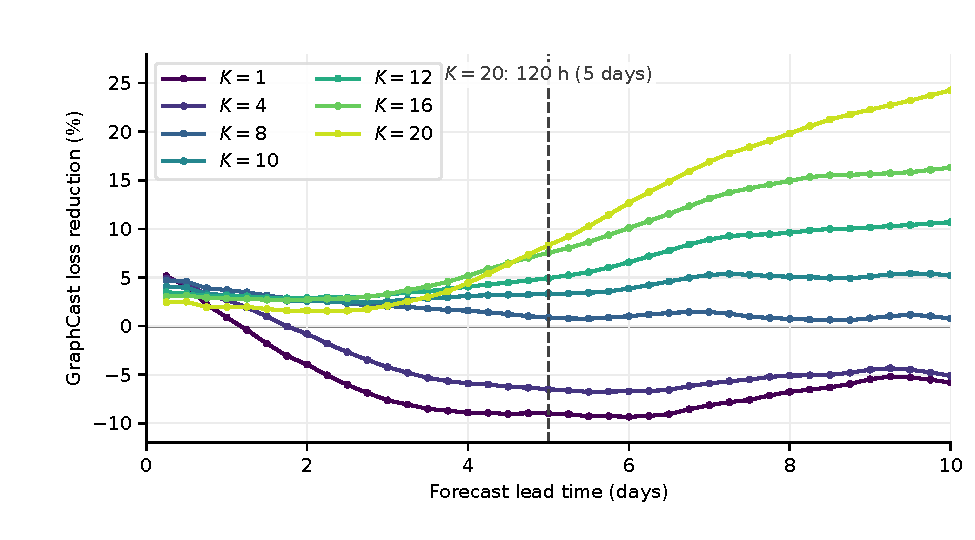
\includegraphics[width=\linewidth]{arxiv_pics/fig8_training_horizon_closed_loop_v4.pdf}
    \caption{Forecast skill after closed-loop training with different training tail lengths $K$. During the tail, corrected GraphCast--Mamba predictions supply subsequent inputs. Each curve shows {GraphCast loss} reduction relative to GraphCast over ten forecast days; positive values indicate improvement. {The vertical dashed line marks $20\times6=120$\,h (5 days), the training tail duration for $K=20$. Gains for this model persist beyond its training tail to day 10, twice that duration.}}
    \label{fig:training_horizon_closed_loop}
\end{figure}

Short training tails primarily improve early forecasts. Models trained with $K=1$ and $K=4$ reduce error during the first one to two days but increase it thereafter, whereas longer training tails yield substantial gains at longer lead times. At day 10, the error reduction relative to GraphCast increases from 5.2\% for $K=10$ to 24.3\% for $K=20$. These curves reveal a crossover: shorter tails favor early forecast skill, while longer tails become more effective as the forecast advances. To examine this crossover in a more controlled setting, we remove correction feedback and train the Mamba correction branch on precomputed forecast trajectories from the frozen GraphCast backbone. In this open-loop setting, corrections do not affect subsequent backbone predictions. As shown in the next section, the crossover becomes more pronounced under this training scheme.

\clearpage
\subsection{Open-loop training and a sharper crossover}
In \emph{open-loop training}, the teacher-forced prefix is followed by a tail driven by the uncorrected GraphCast forecasts. The correction branch learns along this trajectory, but its predictions do not alter subsequent meteorological inputs. Thus, open loop refers to the absence of correction feedback, while teacher forcing refers to the use of ERA5 inputs in the prefix.

In our experiments, training with this teacher-forced prefix and a tail independent of the learned correction was more stable but {yielded smaller improvements at longer lead times}. Figure~\ref{fig:training_horizon_open_loop} shows that short-tail models remain close to GraphCast at long lead times, avoiding the substantial degradation seen in the closed-loop comparison. The crossover is more pronounced here: long-lead gains change markedly between $K=16$ and $K=18$ and increase further for $K=20$ and $K=22$.

\begin{figure}[!htbp]
    \centering
    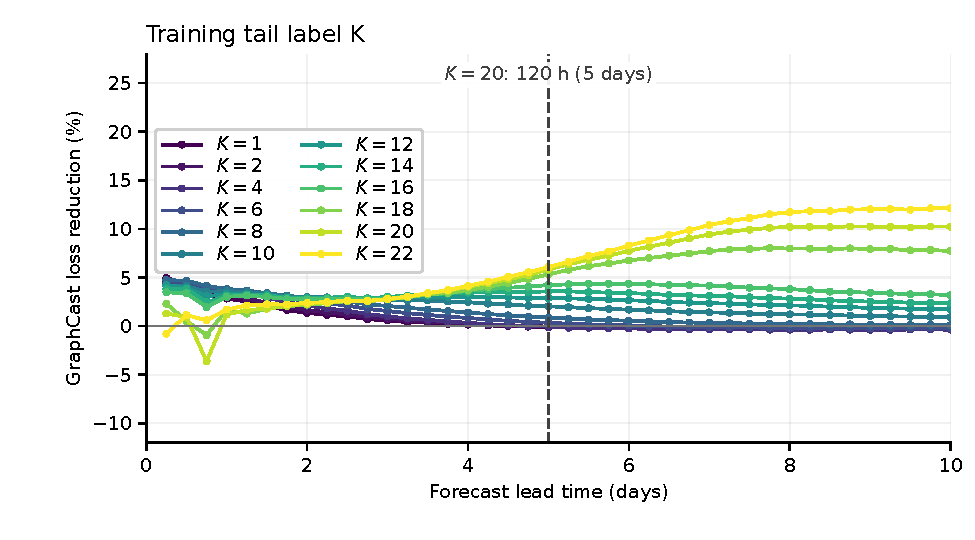
\includegraphics[width=\linewidth]{arxiv_pics/fig9_training_horizon_open_loop_v4.pdf}
    \caption{Forecast skill after open-loop training with a teacher-forced prefix and different training tail lengths $K$. During the tail, uncorrected GraphCast forecasts supply subsequent inputs. {GraphCast loss} reduction exhibits a pronounced crossover, with substantially larger long-lead gains for $K\geq18$. {The vertical dashed line marks $20\times6=120$\,h (5 days), the training tail duration for $K=20$; this model retains positive gains beyond that duration, up to day 10.} This figure and Figure~\ref{fig:training_horizon_closed_loop} use the same vertical scale but compare separate sweeps with different experimental settings and loss reconstructions (Appendix~\ref{app:training_loss}).}
    \label{fig:training_horizon_open_loop}
\end{figure}

This crossover raises an interesting question about how temporal memory, training tail length, and feedback interact. Its mechanism, including why it is sharper under open-loop training, remains unclear. We regard it as an empirical finding that motivates further investigation, rather than evidence for a universal critical value of $K$.


\clearpage
\begingroup\color{blue}
\section{\vfourred{Smoothing controls and scale-dependent diagnostics}}
\label{app:smoothing}

\ifvfivechanges
\par\begingroup\color{vfiveDeleted}\noindent
\sout{This appendix defines the output filter and spectral metrics used in Section~\mbox{\ref{sec:smoothing}}, then provides the loss curves, variable-specific diagnostics, and physical power spectra. Training and memory handling are specified in Appendix~\mbox{\ref{app:training_configuration}}; Table~\mbox{\ref{tab:smoothing_scores}} reports the aggregate comparisons.}
\par\endgroup
\fi
\vfiveadded{This appendix defines the output filter and spectral metrics used in Section~\ref{sec:smoothing}, then provides the loss curves and diagnostics by variable and lead. Training and memory handling are specified in Appendix~\ref{app:training_configuration}; Table~\ref{tab:smoothing_scores} reports the aggregate comparisons.}

\paragraph{\vfourred{Diagnostic protocol.}}
% Prior spectral draft wording, retained internally:
% \vfourred{We compare raw GraphCast, development-filtered GraphCast, and the original M1 and matched reset/reset SWA checkpoints on 36 initializations, every third day at 00\,UTC from 1 January to 16 April 2023, over 40 six-hour leads. The filter is fitted on 32 development initializations in 2022 and changes only GraphCast's reported outputs; all forecasts retain their own unfiltered autoregressive feedback, and neither correction model is amplitude-rescaled. This fixed spectral cohort is separate from the 122-date evaluation and five-seed replication in Appendices~\ref{app:memory_evaluation}--\ref{app:seed_replication}. Its scores are descriptive point estimates, without date-sampling, training-seed, or between-year uncertainty estimates.}
\vfourred{The spectral comparison uses all 122 evaluation initializations and 40 six-hour leads in Section~\ref{sec:eval_protocol}, with the original M1 and matched \vfiveRone{reset/reset} SWA checkpoints. The filter is fitted only on the 2022 development set and changes GraphCast's reported outputs; forecasts retain their own unfiltered autoregressive feedback, and neither correction model is amplitude-rescaled.}
% ANNUAL SPECTRAL PROVENANCE: 122 initializations, every third day at 00 UTC
% from 1 January through 30 December 2023, with 40 six-hour leads.
% Source: artifacts/evaluations/v24_matched_spectra_v5_replot_20261115/.
% Portable exports: archive/Graphs/v5_spectral_matched122_20261115/.
% Earlier 36- and 70-date artifacts remain archived separately.
% Spectral scores are fixed-checkpoint point estimates. The intervals in
% A.4/A.5 belong to their own evaluations and are not transferred here.

\paragraph{\vfourred{Degree-wise least-squares output filter.}}
\vfourred{Following \citet[Supplementary Section~7.4.2]{lam2023graphcast}, we use normalized spherical analysis/synthesis at $1^\circ$ resolution through degree $L=179$. Let $\widehat f_{s,c,k,\ell m}$ and $\widehat y_{s,c,k,\ell m}$ denote forecast and ERA5 coefficients for initialization $s$, variable/pressure channel $c$, lead $k$, degree $\ell$, and order $m$. The fitted gain is}
\vfourred{\begin{equation}
g_{c,k,\ell}=
\frac{\sum_{s\in\mathrm{dev}}\sum_m
       \operatorname{Re}(\widehat f_{s,c,k,\ell m}\widehat y_{s,c,k,\ell m}^{\,*})}
     {\sum_{s\in\mathrm{dev}}\sum_m |\widehat f_{s,c,k,\ell m}|^2}.
\label{eq:spectral_filter}
\end{equation}}
\vfourred{Gains are fitted separately at every lead, channel, and degree, including degree zero, and frozen before 2023 evaluation. They are unrestricted real values; zero denominators receive a recorded identity gain. The filter minimizes coefficient-domain squared error within this isotropic linear family. For analysis $A$ and synthesis $S$, comparing the raw field $f$, unit-gain reconstruction $S[A f]$, and filtered field $S[g A f]$ separates truncation from fitted changes. Reconstruction omits the unrepresented residual, so filtering need not improve native-grid loss at every lead. We evaluate that loss against the original ERA5 fields using Appendix~\ref{app:training_loss}.}

\paragraph{\vfourred{Power, amplitude, and coherence.}}
\vfourred{At each channel and lead, define date-pooled powers $P^f_\ell=\langle\sum_m|\widehat f_{\ell m}|^2\rangle_s$ and $P^y_\ell=\langle\sum_m|\widehat y_{\ell m}|^2\rangle_s$, and cross-power $C_\ell=\langle\sum_m\operatorname{Re}(\widehat f_{\ell m}\widehat y_{\ell m}^{\,*})\rangle_s$. Following \citet{subich2025spectral}, amplitude ratio and coherence satisfy}
\vfourred{\begin{equation}
a_\ell=\sqrt{P^f_\ell/P^y_\ell},\qquad
\rho_\ell=\frac{C_\ell}{\sqrt{P^f_\ell P^y_\ell}},\qquad
\frac{E_\ell}{P^y_\ell}=a_\ell^2+1-2a_\ell\rho_\ell,
\label{eq:spectral_diagnostics}
\end{equation}}
\vfourred{where $E_\ell=P^f_\ell+P^y_\ell-2C_\ell$ is represented error power. Positive filter gains preserve coherence; negative gains reverse its sign. Thus matching amplitudes alone does not imply matching forecast errors. Spectra use physical fields without climatology subtraction and retain degrees 1--179, with wavelength $40{,}030/\ell$\,km. Aggregate curves average channel-wise ratios with normalized GraphCast variable and pressure-level weights, without difference-standard-deviation normalization; physical powers with different units are not added. These diagnostics do not constitute a numerical comparison with the AMSE model itself.}
% Before clarifying the attenuation reference:
% \vfiveadded{Following the reference used by \citet{subich2025spectral}, the amplitude panels mark $a_\ell=\sqrt{0.75}\simeq0.866$. For an individual channel, this denotes a 25\% power deficit at that scale. On combined curves it is only a reference for the weighted mean amplitude ratio, whose square is not the weighted mean power ratio. It is not a threshold for aggregate mismatch or forecast skill. The supporting data include per-channel crossing diagnostics for 20\%, 25\%, and 30\% power deficits, retaining first-lead censoring and later recrossings; these exploratory crossings do not define a universal forecast horizon.}
\vfiveadded{The $\sqrt{0.75}$ reference is an illustrative choice from the effective-resolution diagnostic of \citet[Section~3.1]{subich2025spectral}. For a single channel, $a_\ell^2=0.75$ means a 25\% power deficit relative to ERA5. The combined curves average $a_\ell$ over channels, and the square of that mean differs from the mean of $a_\ell^2$; the reference therefore compares weighted mean amplitudes. First crossings use the sampled integer degrees without interpolation. Crossing positions are threshold-dependent and should be read alongside the full amplitude and coherence curves, especially when amplitudes recover at finer scales. Using references $\sqrt{0.8}$ and $\sqrt{0.7}$ gives day-5 M1/\vfourchange{R1} first crossings of $14/14$ and $18/19$, respectively, and day-10 crossings of $7/10$ and $9/14$, preserving the qualitative contrast. The supporting data separately retain per-channel crossing times at fixed wavenumbers for 20\%, 25\%, and 30\% power deficits, including first-lead censoring and later recrossings. These exploratory diagnostics do not define a universal forecast horizon or a threshold on aggregate mismatch or skill.}


\vfourred{The power-mismatch score underlying Table~\ref{tab:smoothing_scores} instead weights leads, channels, and degrees equally after pooling dates:}
\vfourred{\begin{equation}
D_P=\frac{100}{40\times83\times179}
       \sum_{k=1}^{40}\sum_{c=1}^{83}\sum_{\ell=1}^{179}
       \left|\frac{P^f_{c,k,\ell}}{P^y_{c,k,\ell}}-1\right|.
\label{eq:relative_power_mismatch}
\end{equation}}
% Before the variable-spectrum revision:
% \vfourred{At a fixed lead, the average covers only the 83 channels and 179 degrees; per-feature annotations fix the channel as well. $D_P$ is a percentage relative-power mismatch, not a fraction of total atmospheric energy or a forecast-error score. Equal degree weights make weak spectral tails influential. Numerical exports also retain the ERA5-power-weighted score $100\sum_\ell|P^f_\ell-P^y_\ell|/\sum_\ell P^y_\ell$.}
\vfiveadded{At a fixed lead, the average covers only the 83 channels and 179 degrees; per-channel scores fix the channel as well. $D_P$ is a percentage relative-power mismatch, not a fraction of total atmospheric energy or a forecast-error score. Equal degree weights make weak spectral tails influential. Numerical exports separately retain the ERA5-power-weighted score $100\sum_\ell|P^f_\ell-P^y_\ell|/\sum_\ell P^y_\ell$ within each physical channel and lead. That supplementary score emphasizes energetic scales and does not replace $D_P$ in Table~\ref{tab:smoothing_scores}.}

% Prior spectral draft wording, retained internally:
% \paragraph{\vfourred{Numerical repeatability.}}
% \vfourred{The original reset/reset evaluation saved losses but not spectral moments. Its spectral rerun uses the same SWA checkpoint and yields approximately $0.06\%$ higher pooled rollout loss than the archived evaluation on these dates, with a maximum individual relative difference of $2.46\%$. These finite differences are retained as repeatability diagnostics.}
% INTERNAL REPEATABILITY: the annual reset spectral rerun's pooled loss is
% 10.359790727055467 versus archived 10.359537610436073 (+0.00244%).
% Maximum individual relative drift is 3.29457% against a 0.1% advisory
% reference. These finite differences remain warnings, not failure gates.
% Full measured diagnostics accompany the annual spectral source manifest.

\begin{table}[!htbp]
    \centering
    \begingroup\color{red}\small
    \setlength{\tabcolsep}{4pt}
    \begin{tabular}{lrrrrrr}
        \toprule
        \multicolumn{7}{c}{Relative error (raw GraphCast = 1) $\downarrow$} \\
        \addlinespace[2pt]
        & \multicolumn{2}{c}{Ten-day rollout} & \multicolumn{2}{c}{Day 5} & \multicolumn{2}{c}{Day 10} \\
        \cmidrule(lr){2-3}\cmidrule(lr){4-5}\cmidrule(lr){6-7}
        Forecast & \shortstack{Relative\\MSE} & \shortstack{Relative\\power\\mismatch} & \shortstack{Relative\\MSE} & \shortstack{Relative\\power\\mismatch} & \shortstack{Relative\\MSE} & \shortstack{Relative\\power\\mismatch} \\
        \midrule
        Raw GraphCast & 1.00 & 1.00 & 1.00 & 1.00 & 1.00 & 1.00 \\
        GraphCast + optimal filter & 0.89 & 1.32 & 0.96 & 1.34 & 0.82 & 1.40 \\
        M1 & 0.86 & 1.14 & 0.94 & 1.13 & 0.78 & 1.28 \\
        \vfiveRone{Reset/reset} & 0.91 & 1.11 & 0.97 & 1.12 & 0.86 & 1.16 \\
        \bottomrule
    \end{tabular}
    \endgroup
% Prior spectral draft wording, retained internally:
%     \caption{\vfourred{Relative errors on the fixed 36-date cohort, expressed as ratios to raw GraphCast: $L/L_{\mathrm{GC}}$ for exact GraphCast MSE and $D_P/D_{P,\mathrm{GC}}$ for aggregate power mismatch. Raw GraphCast is $1$ in every column; lower is better. Rollout scores pool all forty leads. The two metrics are normalized separately and measure distinct quantities; both correction models are unfiltered. Appendix~\ref{app:smoothing} defines $D_P$ and the evaluation procedure. Values are fixed-checkpoint point estimates.}}
    \caption{\vfourred{Relative errors on the 122 evaluation initializations, expressed as ratios to raw GraphCast: $L/L_{\mathrm{GC}}$ for exact GraphCast MSE and $D_P/D_{P,\mathrm{GC}}$ for aggregate power mismatch. Raw GraphCast is $1$ in every column; lower is better. Rollout scores pool all forty leads. The two metrics are normalized separately and measure distinct quantities; both correction models are unfiltered. Appendix~\ref{app:smoothing} defines $D_P$ and the evaluation procedure. Values are fixed-checkpoint point estimates.}}
    \label{tab:smoothing_scores}
\end{table}

\begin{figure}[!htbp]
    \centering
    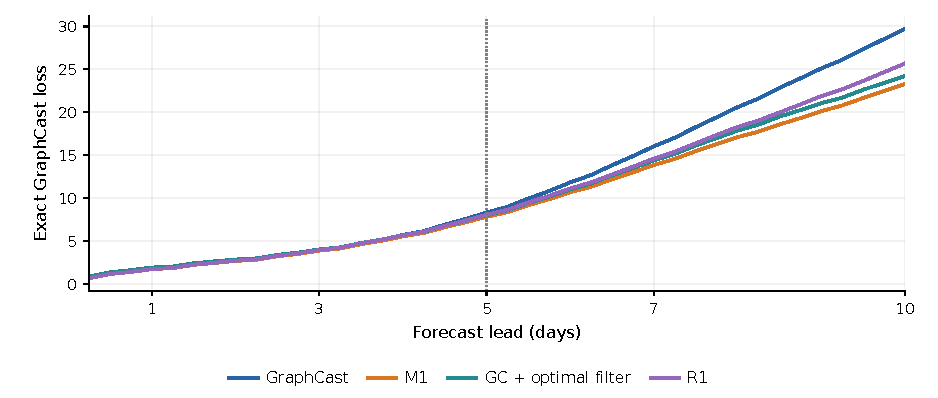
\includegraphics[width=\linewidth]{arxiv_pics/fig10_smoothing_loss_v5_matched122.pdf}
% Prior spectral draft wording, retained internally:
%     \caption{\vfourred{Exact native-grid GraphCast loss for the four predictors on the matched diagnostic cohort. The five-day marker denotes the feedback-conditioned training-tail length. Aggregate scores appear in Table~\ref{tab:smoothing_scores}.}}
    \caption{\vfourred{Exact native-grid GraphCast loss on the 122 evaluation initializations for the four predictors. The five-day marker denotes the feedback-conditioned training-tail length. Aggregate scores appear in Table~\ref{tab:smoothing_scores}.}}
    \label{fig:smoothing_accuracy}
\end{figure}

\subsection{\vfourred{Feature and lead-time diagnostics}}
\label{app:smoothing_features}
\label{app:smoothing_reset}

% Before the variable-spectrum revision:
% \vfourred{Figures~\ref{fig:smoothing_features_amplitude}--\ref{fig:smoothing_leads} resolve the main-text spectral comparison by variable and lead. M1's power attenuation varies across scales, with comparatively modest coherence changes. The full 83-channel breakdown accompanies the figure sources. Raw GraphCast's rollout power mismatch is $59.47\%$, providing the absolute reference for Table~\ref{tab:smoothing_scores}.}
\vfiveadded{Figures~\ref{fig:smoothing_features_day5} and~\ref{fig:smoothing_features_day10} pair amplitude and coherence for $2$\,m temperature (T2m), geopotential at 500\,hPa (Z500), zonal wind at 850\,hPa (U850), and specific humidity at 100\,hPa (Q100). These fields were selected after examining the diagnostics to illustrate retained structure, scale-dependent distortion, an accuracy--attenuation tradeoff, and an adverse case, respectively. They are illustrative rather than a ranking of the 83 channels; the full channel metrics accompany the figure sources. Table~\ref{tab:smoothing_variable_rmse} pairs these spectra with native-grid RMSE for the same dates, checkpoints, and leads.}

% Before interpreting the per-variable reference line:
% \vfiveadded{At day 10, M1 lowers RMSE relative to \vfourchange{R1} by $4.98\%$ for T2m, $4.60\%$ for Z500, and $5.56\%$ for U850, but increases it by $1.01\%$ for Q100. T2m retains comparatively strong spectral amplitude; terrain-related structure can contribute to this behavior~\citep{subich2025spectral}, so it alone does not demonstrate improved dynamics. Z500 shows attenuation at intermediate scales and excess fine-scale power, illustrating why a scalar mismatch is insufficient. U850 combines lower RMSE and improved coherence over some scales with stronger attenuation; Q100 provides a case without a day-10 accuracy benefit.}
\vfiveadded{In these per-variable panels, amplitudes below $\sqrt{0.75}$ identify scales with power more than 25\% below ERA5. The ranges below the line reveal how attenuation varies by field and lead. At day 5, M1 and \vfourchange{R1} exhibit similar behavior: their T2m amplitudes remain above the reference throughout the plotted range, while both U850 curves remain below it from wavenumber $\ell=15$ onward. At day 10, U850 remains below the reference from $\ell=5$ for M1 and $\ell=9$ for \vfourchange{R1}. This level of attenuation therefore extends to coarser scales for M1 despite its lower RMSE and higher coherence over some scales, illustrating an accuracy--attenuation tradeoff.}

\vfiveadded{At day 10, M1 lowers RMSE relative to \vfourchange{R1} by $4.98\%$ for T2m, $4.60\%$ for Z500, and $5.56\%$ for U850, but increases it by $1.01\%$ for Q100. T2m remains largely above the reference, with only isolated dips for M1; terrain-related structure can contribute to its retained amplitude~\citep{subich2025spectral}, so this alone does not demonstrate improved dynamics. Z500's attenuation also extends to coarser scales for M1, but its subsequent fine-scale rise above the reference and unity accompanies low coherence and excess power, not demonstrated recovery of predictable structure. Q100 has intermittent crossings at low wavenumbers, followed by a sustained deficit below the reference from $\ell=11$ for both models; similar attenuation therefore coexists with M1's slightly worse RMSE. These examples motivate reading the full amplitude curves together with coherence and RMSE, rather than treating a first crossing as a sharp boundary of forecast skill.}

\vfiveadded{Across all 83 channels, M1 has lower RMSE than \vfourchange{R1} in 81 channels at each of days 5 and 10. At day 10, however, its equal-degree power mismatch is higher in every channel. These are descriptive fixed-checkpoint comparisons, without channel-wise significance tests. Figure~\ref{fig:smoothing_leads} supplies the combined spectra at six hours, five days, and ten days.}

\vfiveadded{Over all forty leads, M1 has $5.76\%$ lower loss than \vfiveRone{reset/reset}, with power mismatch $67.56\%$ versus $66.06\%$. These aggregate scores do not imply identical spectral fidelity or uniform superiority over \vfiveRone{reset/reset}.}
\begin{table}[!htbp]
    \centering
    \begingroup\color{blue}\small
    \begin{tabular}{lrr}
        \toprule
        & \multicolumn{2}{c}{M1 RMSE reduction relative to R1 (\%) $\uparrow$} \\
        \cmidrule(lr){2-3}
        Field & Day 5 & Day 10 \\
        \midrule
        T2m & 1.37 & 4.98 \\
        Z500 & 2.02 & 4.60 \\
        U850 & 1.76 & 5.56 \\
        Q100 & 0.84 & $-1.01$ \\
        \bottomrule
    \end{tabular}
    \endgroup
    \caption{\vfourred{Native-grid accuracy for the fields in Figures~\ref{fig:smoothing_features_day5} and~\ref{fig:smoothing_features_day10}. Each value is $100(1-\mathrm{RMSE}_{\mathrm{M1}}/\mathrm{RMSE}_{\mathrm{R1}})$; positive values indicate lower M1 RMSE. Physical-unit squared errors are pooled over the 122 dates and area-weighted grid points before taking the square root, separately for each field and lead. These fixed-checkpoint RMSE reductions are distinct from the aggregate GraphCast MSE reductions.}}
    \label{tab:smoothing_variable_rmse}
\end{table}


\begin{figure}[!htbp]
    \centering
% Before the variable-spectrum revision:
%     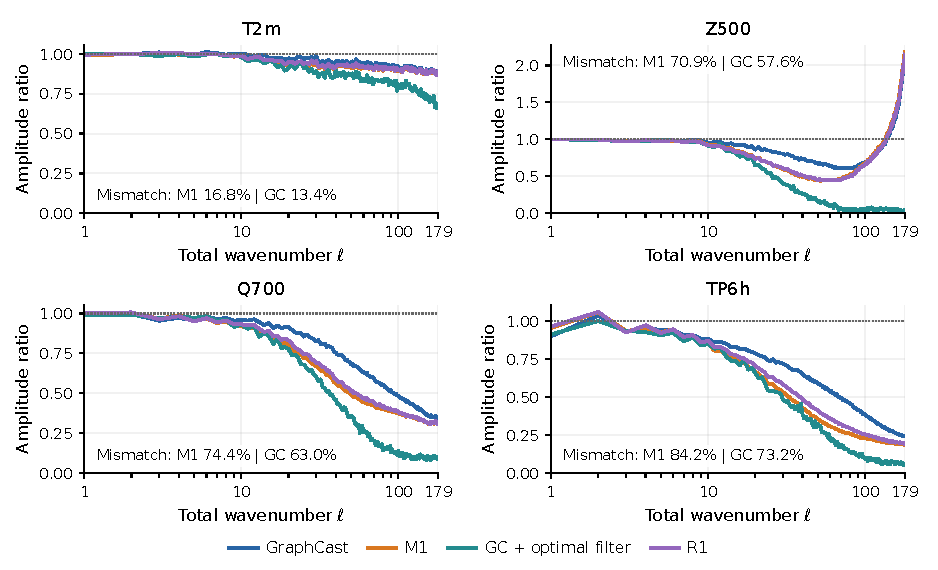
\includegraphics[width=\linewidth]{arxiv_pics/fig11_smoothing_feature_amplitude_v5_matched122.pdf}
    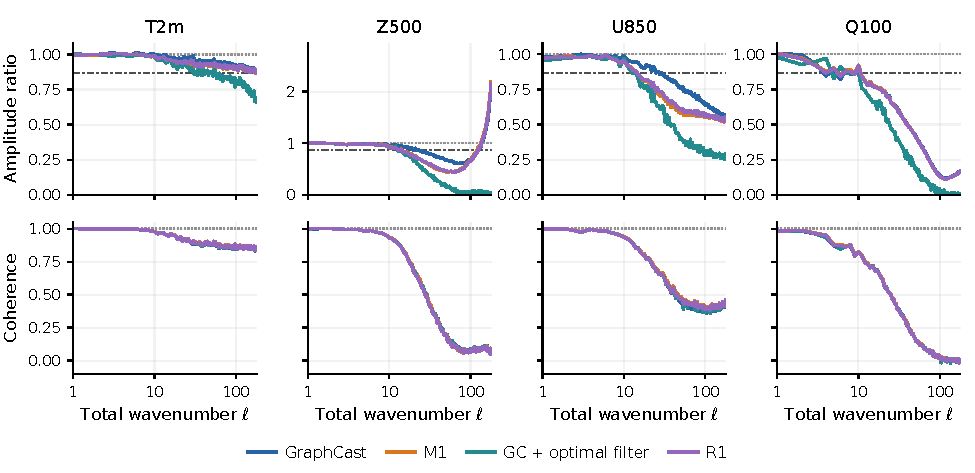
\includegraphics[width=\linewidth]{arxiv_pics/fig11_smoothing_variables_day5_v5_matched122.pdf}
    \caption{\vfourred{Day-5 amplitude ratios (top) and coherence (bottom) for T2m, Z500, U850, and Q100 on the 122 matched initializations. Curves compare raw and filtered GraphCast, M1, and \vfourchange{R1}. The dash-dotted amplitude reference $\sqrt{0.75}$ denotes a 25\% power deficit for an individual field at a given scale; it is not a skill threshold. Amplitude limits vary by field to retain excess fine-scale power. Positive filter gains preserve GraphCast coherence; complementary dashes show coincident curves.}}
    \label{fig:smoothing_features_day5}
% Before the variable-spectrum revision:
%     \caption{\vfourred{Day-5 amplitude ratios for $2$\,m temperature (T2m), geopotential at 500\,hPa (Z500), specific humidity at 700\,hPa (Q700), and six-hour precipitation, comparing raw and filtered GraphCast, M1, and \vfiveRone{reset/reset}. Annotations report the equal-degree power mismatch of M1 and raw GraphCast; lower values indicate closer power matching.}}
% Before the variable-spectrum revision:
%     \label{fig:smoothing_features_amplitude}
\end{figure}

\begin{figure}[!htbp]
    \centering
% Before the variable-spectrum revision:
%     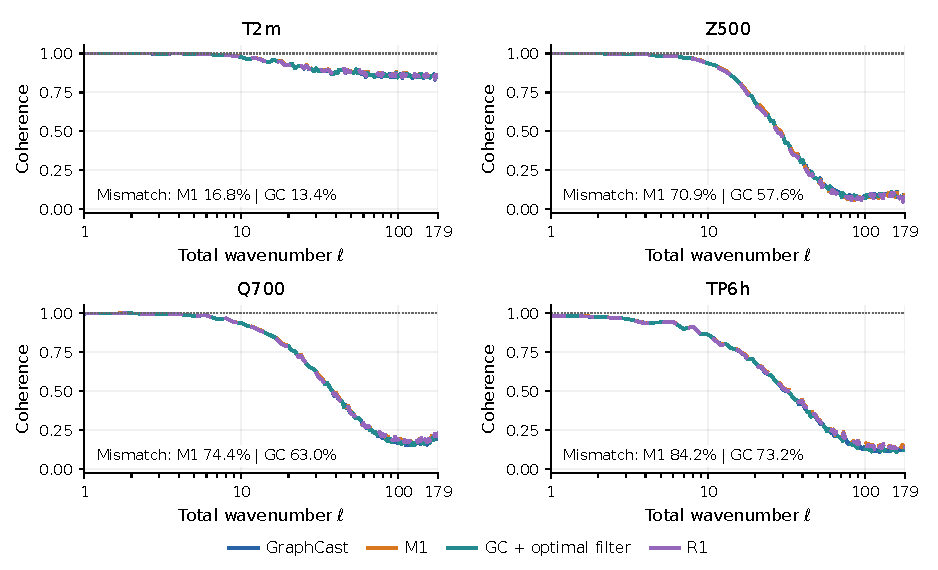
\includegraphics[width=\linewidth]{arxiv_pics/fig12_smoothing_feature_coherence_v5_matched122.pdf}
    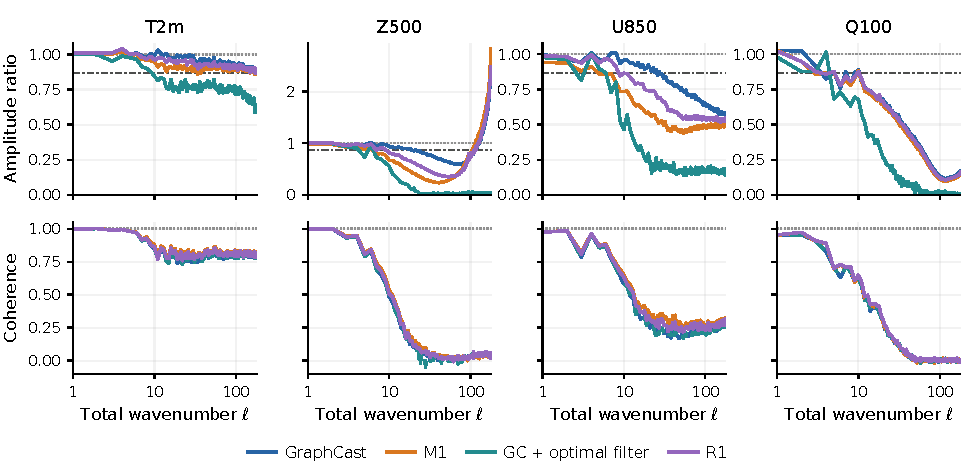
\includegraphics[width=\linewidth]{arxiv_pics/fig12_smoothing_variables_day10_v5_matched122.pdf}
    \caption{\vfourred{Day-10 amplitude ratios (top) and coherence (bottom) for the same forecasts and fields as Figure~\ref{fig:smoothing_features_day5}, using the same axis limits within each field. The longer-lead spectra expose variable- and scale-dependent tradeoffs that the combined curves and aggregate mismatch cannot resolve. Table~\ref{tab:smoothing_variable_rmse} gives the corresponding native-grid RMSE reductions.}}
    \label{fig:smoothing_features_day10}
% Before the variable-spectrum revision:
%     \caption{\vfourred{Coherence for the forecasts and fields in Figure~\ref{fig:smoothing_features_amplitude}. Annotations retain the corresponding power-mismatch scores, which are distinct from coherence.}}
% Before the variable-spectrum revision:
%     \label{fig:smoothing_features_coherence}
\end{figure}

\begin{figure}[!htbp]
    \centering
% Before the variable-spectrum revision:
%     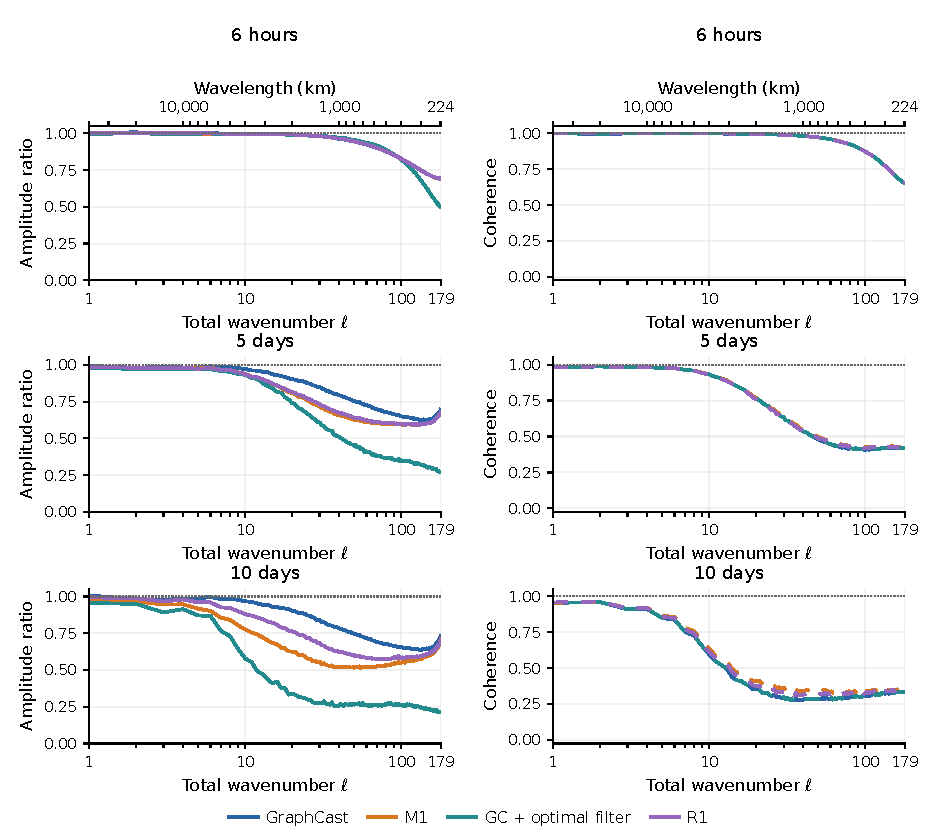
\includegraphics[width=\linewidth]{arxiv_pics/fig13_smoothing_lead_spectra_v5_matched122.pdf}
    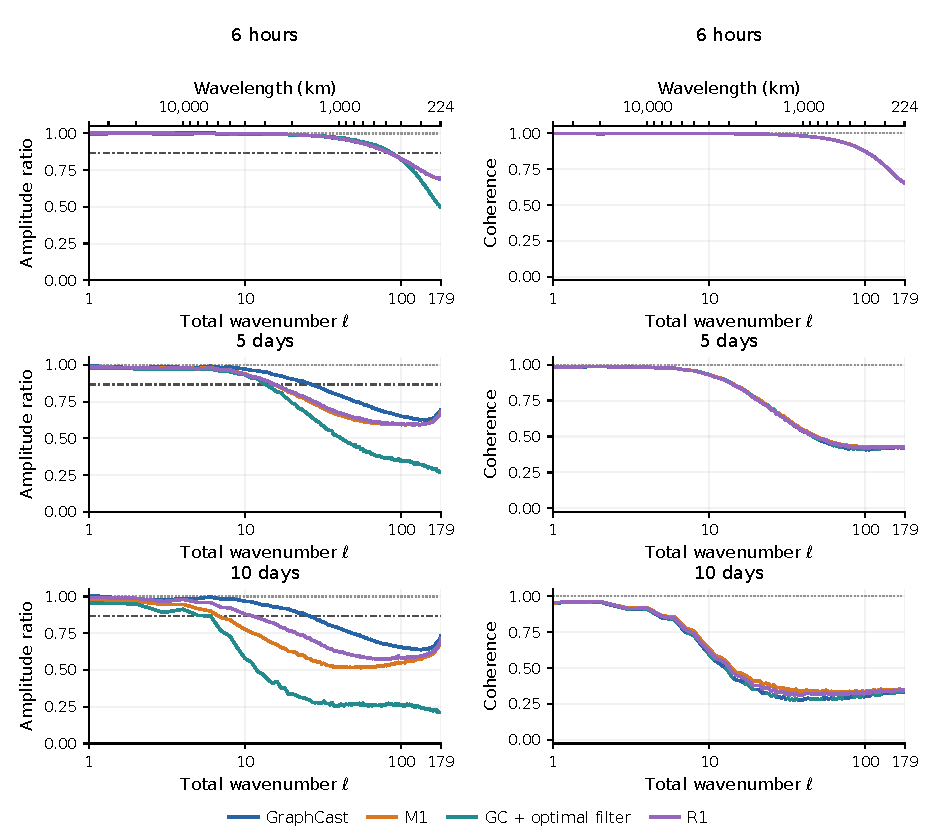
\includegraphics[width=\linewidth]{arxiv_pics/fig13_smoothing_lead_spectra_v5_variables122.pdf}
    \caption{\vfourred{Aggregate amplitude ratio and coherence at six hours, five days, and ten days, using the same 83-channel weighting as Figure~\ref{fig:smoothing_spectra}. The dash-dotted $\sqrt{0.75}$ line is a weighted-amplitude reference, not a threshold on aggregate power loss.}}
% Before the variable-spectrum revision:
%     \caption{\vfourred{Aggregate amplitude ratio and coherence at six hours, five days, and ten days, using the channel weighting defined above.}}
    \label{fig:smoothing_leads}
\end{figure}

\ifvfivechanges
\par\begingroup\color{vfiveDeleted}\noindent
\sout{Matched memory-policy comparison}
\par\noindent
\sout{Former Figures 14 and 15 show the physical power differences underlying the lead-dependent tradeoff in Section~\mbox{\ref{sec:smoothing}}. Over all forty leads, M1 has $6.01\%$ lower loss than reset/reset, with power mismatch $67.14\%$ versus $65.42\%$. The per-field spectra clarify why these aggregate scores do not imply identical spectral fidelity or uniform superiority over reset/reset.}
\par\endgroup
\fi

% Physical-power figure blocks and PDFs are preserved in
% archive/Graphs/v5_removed_power_figures_20261114/.
\ifvfivechanges
\par\noindent\textit{Removed physical power-spectrum figures; former v5 numbers are retained below for review.}\par
\begingroup\color{vfiveDeleted}\noindent
\sout{Former Figure 14 caption: Day-5 physical power spectra for T2m, Z500, Q700, and six-hour precipitation. ERA5 is compared with raw and filtered GraphCast, M1, and reset/reset. Each panel retains its own physical squared units. Powers are pooled over dates; M1 and reset/reset are shown without amplitude rescaling.}
\par\noindent
\sout{Previous day-10 caption: Day-10 physical power spectra for the same forecasts, fields, and conventions as former Figure 14.}
\par\noindent
\sout{Former Figure 15 caption: Day-10 physical power spectra of (a) $2$\,m temperature (T2m), (b) geopotential at 500\,hPa (Z500), (c) specific humidity at 700\,hPa (Q700), and (d) six-hour accumulated precipitation (TP6h). Curves compare ERA5, raw and filtered GraphCast, M1, and reset/reset; each panel shows its variable's physical power units on the vertical axis.}
\par\endgroup
\fi

\ifvfivechanges
\par\noindent\textit{Previous Appendix C prose and captions (consolidated above).}\par
\fi
% Interim-only review material archived internally; not rendered.
% \ifvfivechanges
% \par\begingroup\color{vfiveDeleted}\noindent
% \sout{This appendix provides the filtering method, metric definitions and detailed diagnostics supporting Section~\mbox{\ref{sec:smoothing}}. Figure~\mbox{\ref{fig:smoothing_spectra}} and Table~\mbox{\ref{tab:smoothing_scores}} in the main text summarize day-5 and day-10 spectra and the four-model accuracy--power comparison; the results below use the same fixed 36-date cohort.}
% \par\endgroup
% \fi

\ifvfivechanges
\par\begingroup\color{vfiveDeleted}\noindent
\sout{To distinguish gains attainable through output smoothing from those associated with persistent memory, we compare raw GraphCast, development-filtered GraphCast, M1, and matched reset/reset. Raw GraphCast provides the uncorrected baseline; its filtered output tests what the fitted linear filter can achieve through postprocessing alone. Comparing M1 with this filtered baseline tests whether the learned correction offers an advantage over the smoothing control. Comparing M1 with the separately trained reset/reset model assesses the benefit of retaining memory during training and forecasting, with the architecture and parameter count held fixed.}
\par\endgroup
\fi

% Interim-only review material archived internally; not rendered.
% \ifvfivechanges
% \par\begingroup\color{vfiveDeleted}\noindent
% \sout{The two correction models use the original selected M1 SWA checkpoint and the matched reset/reset SWA checkpoint. All tables and plots use a fixed diagnostic cohort of 36 initializations, every third day at 00\,UTC from 1 January to 16 April 2023, evaluated at 40 six-hour leads. This interim cohort contains completed spectral outputs for every predictor; its data and figure sources are retained as a separate snapshot from subsequent extensions. The GraphCast filter is fitted on the established 32 development initializations in 2022. Each model produces its own autoregressive trajectory; filtering changes only GraphCast's reported output, never the input to the next forecast step. M1 and reset/reset are shown without output filtering or amplitude rescaling. These fixed-checkpoint diagnostics are separate from the principal 122-date evaluation and the five retrainings in Figure~\mbox{\ref{fig:res1_forecast}}.}
% \par\endgroup
% \fi

% Interim-only review material archived internally; not rendered.
% \ifvfivechanges
% \par\begingroup\color{vfiveDeleted}\noindent
% \sout{On these 36 dates, M1 has $4.25\%$ lower ten-day exact GraphCast loss than filtered GraphCast (Figure~\mbox{\ref{fig:smoothing_accuracy}}). Its aggregate relative power mismatch is also lower, $67.14\%$ versus $78.28\%$. Thus M1 improves both measured scores relative to this filtered baseline on the diagnostic cohort. Raw GraphCast retains lower power mismatch, $58.59\%$, alongside higher forecast loss. Table~\mbox{\ref{tab:smoothing_scores}} reports both scores as ratios to raw GraphCast over the rollout and at days 5 and 10 ($1$ denotes the baseline; lower is better). These point estimates concern fixed checkpoints and the tested filter family; they do not identify what fraction of the correction benefit is caused by smoothing. The comparison with reset/reset is discussed separately in Appendix~\mbox{\ref{app:smoothing_reset}}.}
% \par\endgroup
% \fi

% Interim-only review caption retained internally.
% \ifvfivechanges
% \par\begingroup\color{vfiveDeleted}\noindent
% \sout{Previous Figure~\mbox{\ref{fig:smoothing_accuracy}} caption: Exact native-grid GraphCast loss for raw GraphCast, filtered GraphCast, M1 and reset/reset on 36 matched 2023 initializations. Each forecast follows its own unfiltered feedback trajectory. All losses use identical dates and leads. The five-day marker denotes the feedback-conditioned training-tail length. Curves are fixed-checkpoint point estimates without confidence bands.}
% \par\endgroup
% \fi

\ifvfivechanges
\par\begingroup\color{vfiveDeleted}\noindent
\sout{Following the amplitude/coherence diagnostics of \mbox{\citet{subich2025spectral}}, Figure~\mbox{\ref{fig:smoothing_spectra}} separates power matching from pattern agreement. M1 often attenuates more power than raw GraphCast, with comparatively modest coherence changes; the effect varies across variables and scales (Appendix~\mbox{\ref{app:smoothing_features}}). This is consistent with amplitude adjustment contributing to its accuracy gains, while the filtering comparison demonstrates a remaining advantage over the tested postprocessing baseline. The matched training-policy experiment in Section~\mbox{\ref{sec:memory_ablation}} separately supports a contribution from persistent memory; Appendix~\mbox{\ref{app:smoothing_reset}} shows the original M1 and reset/reset spectra on their common diagnostic dates.}
\par\endgroup
\fi

\ifvfivechanges
\par\begingroup\color{vfiveDeleted}\noindent
\sout{Write $A$ and $S$ for analysis and synthesis. For GraphCast, the raw field $f$, the unit-gain reconstruction $S[A f]$, and the filtered field $S[g A f]$ distinguish truncation from fitted amplitude changes. Reconstruction does not restore the unrepresented residual, so coefficient-domain optimization need not improve native-grid loss at every lead. The comparison with M1 and reset/reset uses their original unfiltered fields. All native-grid losses use the original ERA5 fields and the exact GraphCast weighting of Appendix~\mbox{\ref{app:training_loss}}.}
\par\endgroup
\fi

% Interim-only review material archived internally; not rendered.
% \ifvfivechanges
% \par\begingroup\color{vfiveDeleted}\noindent
% \sout{The 36-date cohort supports descriptive comparisons for the evaluated checkpoints and covers January--April rather than a full year. We do not estimate date-sampling confidence intervals, training-seed variation or between-year uncertainty from this diagnostic sample. The paired date-bootstrap intervals and five-seed standard deviations reported elsewhere concern the larger evaluations in Appendices~\mbox{\ref{app:memory_evaluation}} and~\mbox{\ref{app:seed_replication}}; they are not transferred to these curves or scores.}
% \par\endgroup
% \fi

% Interim-only review material archived internally; not rendered.
% \ifvfivechanges
% \par\begingroup\color{vfiveDeleted}\noindent
% \sout{The reset/reset spectral rerun has finite numerical differences from its archived loss evaluation on these same dates: pooled rollout loss is approximately $0.06\%$ higher, with a maximum individual relative difference of $2.46\%$. These measured differences are retained as numerical-repeatability diagnostics. All displayed comparisons use the common 36 dates and the original raw fields for both memory policies.}
% \par\endgroup
% \fi

% Interim-only review material archived internally; not rendered.
% \ifvfivechanges
% \par\begingroup\color{vfiveDeleted}\noindent
% \sout{Figures~\mbox{\ref{fig:smoothing_features_amplitude}} and~\mbox{\ref{fig:smoothing_features_coherence}} show all four predictors for the same fixed diagnostics---T2m, Z500, Q700 and six-hour precipitation---on the common 36-date cohort. These fields span favorable power preservation, scale-dependent departures and strong power deficits. The full 83-channel numerical breakdown accompanies the figure sources. Figure~\mbox{\ref{fig:smoothing_leads}} retains six-hour and day-10 diagnostics alongside day 5; the longer lead remains relevant because the principal accuracy claim extends to ten days. No numerical comparison with the AMSE model itself is implied: we adopt its spectral diagnostics for our own resolution, verification data and checkpoints.}
% \par\endgroup
% \fi

% Interim-only review material archived internally; not rendered.
% \ifvfivechanges
% \par\begingroup\color{vfiveDeleted}\noindent
% \sout{Previous Figure~\mbox{\ref{fig:smoothing_features_amplitude}} caption: Day-5 amplitude ratios for $2$\,m temperature (T2m), geopotential at 500\,hPa (Z500), specific humidity at 700\,hPa (Q700), and six-hour precipitation (TP6h). Every panel includes raw GraphCast, filtered GraphCast, M1 and reset/reset on the same 36 dates. Panel annotations compare the equal-degree power mismatch of M1 and raw GraphCast, with lower values denoting closer power matching. Ratios and mismatch scores are computed from pooled powers.}
% \par\endgroup
% \fi

\ifvfivechanges
\par\begingroup\color{vfiveDeleted}\noindent
\sout{Former Figure 12 caption: Coherence for the same forecasts and fields as former Figure 11. Coherence measures normalized cross-power separately from amplitude fidelity. Panel annotations retain the same M1/raw-GraphCast power-mismatch scores to identify the corresponding spectral-fidelity comparison; they are not coherence errors.}
\par\endgroup
\fi

% Interim-only review material archived internally; not rendered.
% \ifvfivechanges
% \par\begingroup\color{vfiveDeleted}\noindent
% \sout{Previous Figure~\mbox{\ref{fig:smoothing_leads}} caption: Aggregate spectral amplitude and coherence at six hours, five days and ten days for all four predictors on the same 36 dates. Channel-wise ratios are averaged with the same variable/pressure weights as Figure~\mbox{\ref{fig:smoothing_spectra}}. Full degree ranges are retained. These are point estimates without simultaneous significance estimates across scales.}
% \par\endgroup
% \fi

% Interim-only review material archived internally; not rendered.
% \ifvfivechanges
% \par\begingroup\color{vfiveDeleted}\noindent
% \sout{The original matched reset/reset evaluation saved losses but not spectral moments. The diagnostic rerun uses the same reset-trained SWA checkpoint, resetting both its SSM state and convolution cache before every prediction. M1 uses the original selected checkpoint with persistent memory. Table~\mbox{\ref{tab:smoothing_scores}} in the main text and Figures~\mbox{\ref{fig:memory_power_day5}} and~\mbox{\ref{fig:memory_power_day10}} below show these policies together with raw and filtered GraphCast on the same 36 dates used throughout this appendix. The two correction models are shown as predicted, without post-hoc amplitude matching. The 122-date memory-training comparison remains the principal evidence for the training-policy effect.}
% \par\endgroup
% \fi

\ifvfivechanges
\par\begingroup\color{vfiveDeleted}\noindent
\sout{At day 5, M1 achieves $2.84\%$ lower GraphCast-weighted MSE than reset/reset, while aggregate power mismatch is $68.66\%$ versus $68.16\%$, a difference of $0.50$ percentage points. Thus, at this lead, persistent memory provides an accuracy benefit with a limited change in the aggregate power-mismatch score. Similar aggregate scores do not imply identical spectra: the per-field power and coherence curves retain differences across scales.}
\par\endgroup
\fi

\ifvfivechanges
\par\begingroup\color{vfiveDeleted}\noindent
\sout{At day 10, the MSE advantage increases to $10.20\%$, accompanied by a larger power-mismatch difference: $84.47\%$ versus $75.74\%$. All four forecasts have higher absolute MSE and lower aggregate spectral coherence than at day 5 (Figures~\mbox{\ref{fig:smoothing_accuracy}} and~\mbox{\ref{fig:smoothing_leads}}). This lead extends beyond the five-day ($K=20$) feedback-conditioned training tail and illustrates the evolving accuracy--spectral-fidelity tradeoff during longer rollouts. It remains relevant to the paper's ten-day forecasting results. Averaged over all forty leads, M1 has $6.01\%$ lower loss, with power mismatch $67.14\%$ versus $65.42\%$. These results support a lead-dependent accuracy benefit; they do not establish an improvement at identical spectral fidelity or a uniformly better tradeoff than reset/reset. Table~\mbox{\ref{tab:smoothing_scores}} summarizes the separate loss and power-mismatch ratios relative to raw GraphCast for all four predictors ($1$ denotes the baseline; lower is better).}
\par\endgroup
\fi

\ifvfivechanges
\par\begingroup\color{vfiveDeleted}\noindent
\sout{Former Figures 14 and 15 show the corresponding physical power spectra for T2m, Z500, Q700 and six-hour precipitation. ERA5 provides the reference in each panel. Showing M1 and reset/reset together makes their power differences visible without combining variables with different units or interpreting a single aggregate mismatch as an identical spectrum.}
\par\endgroup
\fi

% Interim-only review material archived internally; not rendered.
% \ifvfivechanges
% \par\begingroup\color{vfiveDeleted}\noindent
% \sout{Previous Figure~\mbox{\ref{fig:memory_power_day5}} caption: Day-5 physical power spectra of the original M1 and reset/reset forecasts, with raw GraphCast, filtered GraphCast and ERA5, on the same 36 dates as Table~\mbox{\ref{tab:smoothing_scores}}. Each panel retains its own physical squared units. Powers are pooled over dates before plotting; degree zero is omitted and no climatology is subtracted. Both memory policies are shown without amplitude rescaling.}
% \par\endgroup
% \fi

% Interim-only review material archived internally; not rendered.
% \ifvfivechanges
% \par\begingroup\color{vfiveDeleted}\noindent
% \sout{Previous Figure~\mbox{\ref{fig:memory_power_day10}} caption: Day-10 physical power spectra for the same forecasts, dates, fields and conventions as Figure~\mbox{\ref{fig:memory_power_day5}}. These spectra accompany the $10.20\%$ lower exact native-grid loss of M1 relative to reset/reset at this lead on the 36-date cohort. The plotted power differences remain part of the original predictions.}
% \par\endgroup
% \fi

\ifvfivechanges
\par\noindent\textit{Earlier pilot deletions retained for review.}\par
\fi
% Interim-only review material archived internally; not rendered.
% \ifvfivechanges
% \par\begingroup\color{vfiveDeleted}\noindent
% \sout{On these 36 dates, carry/carry has $4.25\%$ lower ten-day exact GraphCast loss than filtered GraphCast (Figure~\mbox{\ref{fig:smoothing_accuracy}}). Its aggregate relative power mismatch is also lower, $67.14\%$ versus $78.28\%$. Thus carry/carry improves both measured scores relative to this filtered baseline on the diagnostic cohort. Raw GraphCast retains lower power mismatch, $58.59\%$, alongside higher forecast loss. Table~\mbox{\ref{tab:smoothing_scores}} reports both scores as reductions relative to raw GraphCast over the rollout and at days 5 and 10. These point estimates concern fixed checkpoints and the tested filter family; they do not identify what fraction of the correction benefit is caused by smoothing. The comparison with reset/reset is discussed separately in Appendix~\mbox{\ref{app:smoothing_reset}}.}
% \par\endgroup
% \fi

\ifvfivechanges
\par\begingroup\color{vfiveDeleted}\noindent
\sout{At day 10, the MSE advantage increases to $10.20\%$, accompanied by a larger power-mismatch difference: $84.47\%$ versus $75.74\%$. All four forecasts have higher absolute MSE and lower aggregate spectral coherence than at day 5 (Figures~\mbox{\ref{fig:smoothing_accuracy}} and~\mbox{\ref{fig:smoothing_leads}}). This lead extends beyond the five-day ($K=20$) feedback-conditioned training tail and illustrates the evolving accuracy--spectral-fidelity tradeoff during longer rollouts. It remains relevant to the paper's ten-day forecasting results. Averaged over all forty leads, carry/carry has $6.01\%$ lower loss, with power mismatch $67.14\%$ versus $65.42\%$. These results support a lead-dependent accuracy benefit; they do not establish an improvement at identical spectral fidelity or a uniformly better tradeoff than reset/reset. Table~\mbox{\ref{tab:smoothing_scores}} summarizes the separate loss and power-mismatch reductions relative to raw GraphCast for all four predictors.}
\par\endgroup
\fi
\endgroup

\clearpage

\section{Comparison on a common verification grid}
\label{app:common_grid}
\begin{figure}[!t]
    \centering
    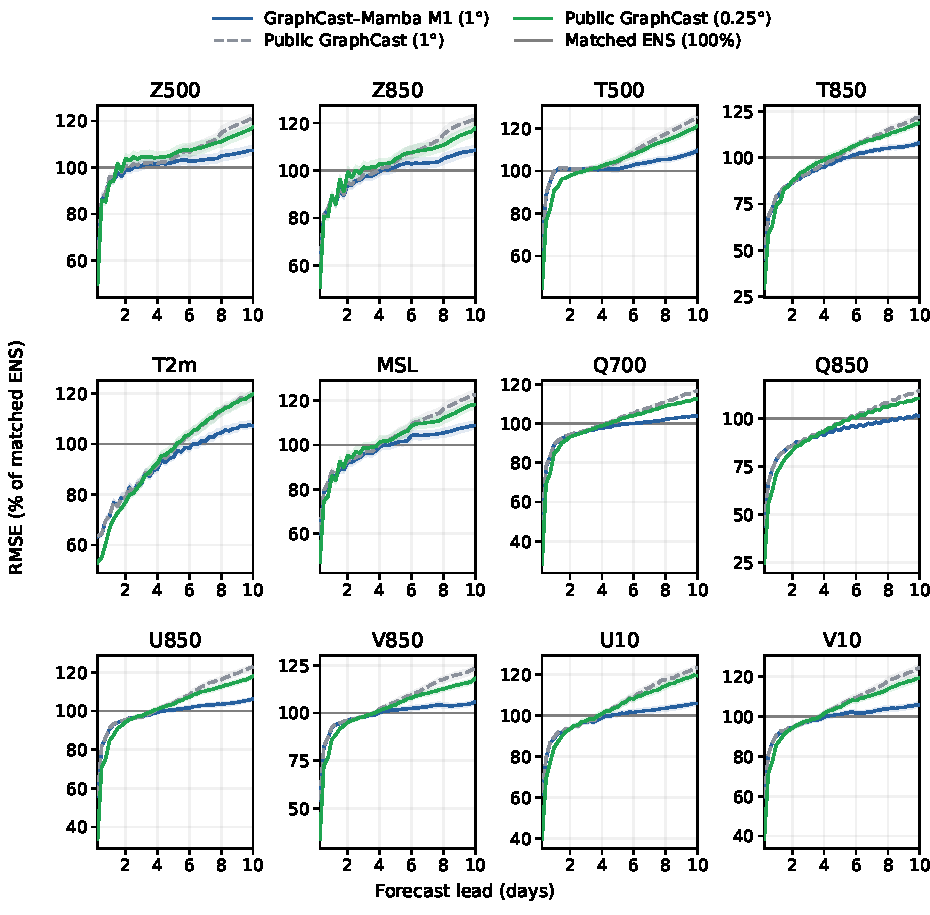
\includegraphics[width=\linewidth]{arxiv_pics/fig14_common_grid_all_variables_v5_ci.pdf}
    \caption{\vfourchange{The comparison in Figure~\ref{fig:common_grid_selected} extended to 12 diagnostics. Blue shows the selected \mbox{GraphCast--Mamba} model M1 ($1^\circ$), dashed gray its public GraphCast\_small backbone ($1^\circ$), and green the public GraphCast checkpoint ($0.25^\circ$). Z denotes geopotential, T temperature, Q specific humidity, U zonal wind, and V meridional wind; a three-digit suffix gives pressure in hPa. T2m denotes $2$\,m temperature, U10 and V10 the $10$\,m wind components, and MSL mean sea-level pressure. All four forecasts use identical dates and ERA5 truth at each diagnostic and lead on the $1.5^\circ$ grid; the available date set varies across points (91--108 starts). Curves show pooled RMSE as a percentage of the matched ENS-mean RMSE, with ENS at $100\%$. Shading gives pointwise 95\% date-block-bootstrap intervals, conditional on the fixed checkpoints.}}
    \label{fig:res1_all_variables}
\end{figure}


\paragraph{\vfourchange{Models and forecast protocol.}}
\ifvfivechanges
\par\begingroup\color{vfiveDeleted}\noindent
\sout{All three GraphCast-based forecasts are generated locally from fixed checkpoints. M1 is the same selected correction used in the principal evaluation, trained on 2015--2021 and selected on 2022 development data. Its frozen backbone is the public DeepMind GraphCast\_small checkpoint trained on ERA5 1979--2015, with a $1^\circ$ grid, 13 pressure levels and mesh refinement level 5. The higher-resolution reference is the public GraphCast checkpoint trained on ERA5 1979--2017, with a $0.25^\circ$ grid, 37 levels and mesh refinement level 6. Both public checkpoints include precipitation as an input and output and use the supplied GraphCast normalization statistics. Their grids contain $181\times360$ and $721\times1440$ points, respectively. Their meshes contain 10,242 and 40,962 vertices, respectively. The higher-resolution model therefore operates on much larger spatial graphs; the computational comparison concerns FLOPs and activation memory. Exact checkpoint filenames, checksums and configuration are recorded in the figure-source manifest.}
\par\endgroup
\fi
\vfourchange{The locally generated forecasts compare M1 (Appendix~\ref{app:training_configuration}), its public GraphCast\_small backbone, and public $0.25^\circ$ GraphCast. GraphCast\_small was trained on ERA5 1979--2015, uses 13 pressure levels and mesh refinement level 5, and has $181\times360$ grid points and 10,242 mesh vertices. The higher-resolution checkpoint was trained on ERA5 1979--2017, uses 37 levels and refinement level 6, and has $721\times1440$ grid points and 40,962 mesh vertices. Both include precipitation as input and output and use supplied GraphCast normalization statistics. Checkpoint identifiers and checksums are retained with the figure sources.}

\ifvfivechanges
\par\begingroup\color{vfiveDeleted}\noindent
\sout{Each forecast receives observed ERA5 states at $-6$ and $0$\,h, then advances through 40 six-hour leads from 6 to 240\,h using its own forecast feedback. Time-varying $0.25^\circ$ ERA5 inputs are subsampled to $1^\circ$ for GraphCast\_small and M1 and restricted to their 13 pressure levels; these models retain static fields from their existing training and evaluation store. M1 begins each forecast with zero temporal memory and feeds back its full corrected prediction. Network inference uses bfloat16, with physical fields and state boundaries in float32.}
\par\endgroup
\fi
\vfourchange{Forecast initialization and autoregressive feedback follow Section~\ref{sec:eval_protocol}. For GraphCast\_small and M1, time-varying ERA5 inputs use the $1^\circ$/13-level subsampling of Appendix~\ref{app:training_configuration}, with static fields retained from their training/evaluation store. All network inference uses bfloat16 with float32 physical fields and state boundaries.}

\paragraph{\vfourchange{Dates and ENS reference.}}
\ifvfivechanges
\par\begingroup\color{vfiveDeleted}\noindent
\sout{The candidate sample consists of 122 initializations at 00\,UTC every third day from 1 January through 30 December 2023, with verification extending through 9 January 2024. ENS denotes the ECMWF IFS ensemble-mean forecast distributed by WeatherBench~2 on its conservative $121\times240$ grid. We use available 2023 forecasts from the extended 2016--2024 store.}\footnote{\raggedright The ENS stores under \url{gs://weatherbench2/datasets/ifs_ens/} are \path{2016-2024-240x121_equiangular_with_poles_conservative_mean.zarr} (forecast source) and \path{2018-2022-240x121_equiangular_with_poles_conservative_mean.zarr} (layout reference).}\sout{ Missing metadata and coordinate arrays were reconstructed from the complete 2018--2022 sibling store, with decoding checked against 71 overlapping forecast chunks. Missing forecast chunks remain unavailable.}
\par\endgroup
\fi
\vfourchange{The candidate dates follow the 122-start evaluation grid in Section~\ref{sec:eval_protocol}, with verification extending through 9 January 2024. ENS is the ECMWF IFS ensemble mean distributed by WeatherBench~2 on its conservative $121\times240$ grid; we use available 2023 forecasts from the 2016--2024 archive. Missing metadata and coordinate arrays were reconstructed from its complete 2018--2022 sibling, with decoding checked against 71 overlapping forecast chunks. Missing forecast chunks remain unavailable.}
% ENS source provenance: gs://weatherbench2/datasets/ifs_ens/
% Forecast source: 2016-2024-240x121_equiangular_with_poles_conservative_mean.zarr
% Metadata/layout reference: 2018-2022-240x121_equiangular_with_poles_conservative_mean.zarr

\vfourchange{At each diagnostic and lead, we retain exactly the same ENS-available initializations for all four forecasts. This gives 91--108 starts per point across the 12 diagnostics (92--105 in Figure~\ref{fig:common_grid_selected}), with 46,930 initialization--lead--diagnostic combinations per model. The matched date set can vary between diagnostics and leads; there is no single complete subset underlying every point. Selection depends only on forecast availability, not errors. Availability masks and the full candidate manifest accompany the figures.}

\paragraph{\vfourchange{Verification and metric.}}
\vfourchange{Every forecast is verified against identical ERA5 fields~\citep{hersbach2020era5} from ARCO ERA5, with source-data repairs validated against the independently curated NSF NCAR ERA5 archive. Native model predictions and $0.25^\circ$ verification fields are remapped to the common $1.5^\circ$ grid using first-order conservative spherical-cell overlap with periodic longitude; the archived ENS fields already occupy this grid. For each diagnostic and lead, we compute spatial mean squared errors with normalized cosine-latitude weights, average equally over the matched starts, and take the square root. The plotted value is $100\,\mathrm{RMSE}_{\mathrm{model}}/\mathrm{RMSE}_{\mathrm{ENS}}$, with identical dates in numerator and denominator. These physical-unit RMSE diagnostics are separate from the normalized GraphCast training loss.}

\paragraph{\vfourchange{Paired uncertainty over forecast dates.}}
\ifvfivechanges
\par\begingroup\color{vfiveDeleted}\noindent
\sout{We use 10,000 non-wrapping moving-block-bootstrap draws with seed 20260916 and blocks of five consecutive positions on the original regular 122-date grid (12 elapsed days). A draw concatenates sampled blocks and truncates to 122 positions. The same draw is applied jointly to all four forecasts, and each diagnostic--lead ENS-availability mask is applied after resampling. For each draw we pool spatial MSE over the retained sampled dates, take square roots, and compute model/ENS RMSE ratios. Shading in Figures~\mbox{\ref{fig:common_grid_selected}} and~\mbox{\ref{fig:res1_all_variables}} shows the 2.5th and 97.5th percentiles. ENS is exactly $100\%$ by definition. Table~\mbox{\ref{tab:common_grid_intervals}} instead reports paired intervals for $100(1-\mathrm{RMSE}_{\mathrm{M1}}/\mathrm{RMSE}_{0.25^\circ})$ at day 10, using the same draws. Pairing accounts for shared weather variability; overlap of separate model bands is not a test of their difference.}
\par\endgroup
\fi
\vfourchange{We use the paired block-bootstrap procedure of Appendix~\ref{app:memory_evaluation}, applying each draw jointly to all four forecasts before applying the diagnostic--lead ENS-availability masks. Within each draw, squared errors are pooled over retained dates before computing RMSE and model/ENS ratios; ENS is $100\%$ by definition. The percentile intervals form the shading in Figures~\ref{fig:common_grid_selected} and~\ref{fig:res1_all_variables}. Table~\ref{tab:common_grid_intervals} uses the same draws for $100(1-\mathrm{RMSE}_{\mathrm{M1}}/\mathrm{RMSE}_{0.25^\circ})$ at day 10. This paired contrast accounts for shared weather; overlap of separate model bands does not test their difference.}

\ifvfivechanges
\par\begingroup\color{vfiveDeleted}\noindent
\sout{These are pointwise intervals conditional on the fixed checkpoints, observed year and availability masks. They quantify neither training-seed nor between-year variation, and are not simultaneous intervals across diagnostics or leads. Overlapping forecast windows and seasonal dependence limit the effective sample size; the chosen blocks retain some dependence without guaranteeing exact nominal coverage. Non-wrapping blocks underweight boundary dates. No new forecasts are generated for this uncertainty analysis.}
\par\endgroup
\fi
\vfourchange{These intervals additionally condition on ENS-availability masks and are pointwise across diagnostics as well as leads. The uncertainty scope and overlap/boundary limitations in Appendix~\ref{app:memory_evaluation} apply; seasonal dependence also limits the bootstrap approximation.}

\begin{table}[!htbp]
    \centering
    \small
    \begingroup\color{blue}
    \begin{tabular}{lrrr}
        \toprule
        Diagnostic & Matched starts & RMSE reduction (\%) & Pointwise 95\% interval (\%) \\
        \midrule
        Z500 & 91 & 8.48 & [6.54, 10.02] \\
        Z850 & 91 & 7.91 & [6.03, 9.56] \\
        T500 & 104 & 9.38 & [8.23, 10.36] \\
        T850 & 104 & 8.91 & [7.67, 9.89] \\
        T2m & 98 & 10.58 & [8.82, 11.55] \\
        MSL & 97 & 8.00 & [6.09, 9.48] \\
        Q700 & 94 & 7.70 & [6.93, 8.45] \\
        Q850 & 94 & 8.27 & [7.57, 8.90] \\
        U850 & 98 & 9.83 & [8.67, 10.80] \\
        V850 & 99 & 10.42 & [9.04, 11.68] \\
        U10 & 97 & 11.42 & [10.50, 12.27] \\
        V10 & 106 & 11.21 & [9.84, 12.45] \\
        \bottomrule
    \end{tabular}
    \endgroup
    \caption{\vfourchange{Day-10 RMSE reduction of the original selected M1 relative to public $0.25^\circ$ GraphCast on the common $1.5^\circ$ grid. Each diagnostic uses identical ENS-available dates for both models. Paired date-block-bootstrap intervals concern fixed checkpoints and are pointwise, without adjustment across the 12 diagnostics.}}
    \label{tab:common_grid_intervals}
\end{table}

\FloatBarrier
\paragraph{\vfourchange{Interpretation.}}
\ifvfivechanges
\par\begingroup\color{vfiveDeleted}\noindent
\sout{The figures show point estimates and pointwise date-sampling intervals for the specified fixed checkpoints on the available matched samples; these do not measure training-seed variation or simultaneous significance across diagnostics and leads. Ten-day verification windows overlap, so the starts are not independent weather realizations. Checkpoints also differ in architecture, pressure levels and training coverage; their comparison does not isolate resolution or attribute the full advantage to memory. The matched memory controls in Section~\mbox{\ref{sec:memory_ablation}} address the latter question. Lower RMSE after common-grid remapping establishes neither finer-scale skill at $0.25^\circ$ nor a measured inference speedup. At day 10, M1 has lower RMSE than the public $0.25^\circ$ checkpoint on all 12 diagnostics, but higher RMSE than ENS.}
\par\endgroup
\fi
\vfourchange{The checkpoints differ in architecture, pressure levels, and training coverage, so this comparison does not isolate resolution or attribute the full advantage to memory; Section~\ref{sec:memory_ablation} addresses memory with a matched control. Lower RMSE after common-grid remapping establishes neither finer-scale skill at $0.25^\circ$ nor a measured inference speedup. At day 10, M1 has lower RMSE than public $0.25^\circ$ GraphCast on all 12 diagnostics, while ENS remains better.}

\clearpage
\section{Forecast examples at city locations}
\label{app:city_traces}
To complement the aggregate seven-year results in Section~\ref{sec:numerical}, Figure~\ref{fig:city_traces_jan} illustrates local forecast behavior for temperature, wind, and precipitation at Paris and New York City. These examples use a separate correction trained on 15 years of ERA5 data (2007--2021), with the configuration specified in the figure caption. Over 120--240\,h, the correction reduces mean absolute error (MAE) in four of the six displayed city--variable pairs. Errors increase for Paris temperature and New York precipitation, illustrating that aggregate skill gains can coexist with deterioration in individual forecasts.

\begin{figure}[!htbp]
    \centering
    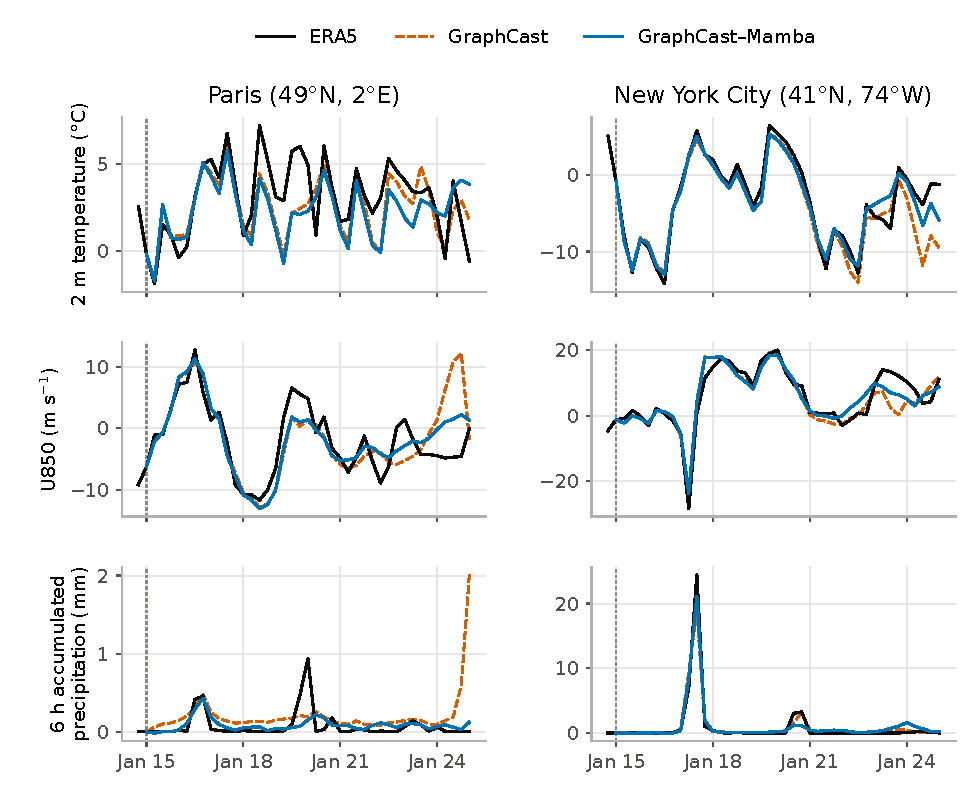
\includegraphics[width=\linewidth]{arxiv_pics/fig15_city_forecasts_v5.pdf}
    \caption{{Ten-day forecasts from 00\,UTC on 15 January 2022 at the $1^\circ$ grid points nearest Paris ($49^\circ$N, $2^\circ$E; left) and New York City ($41^\circ$N, $74^\circ$W; right).
    From top to bottom, rows show $2$\,m temperature (T2m), $850$\,hPa zonal wind (U850), and $6$\,h accumulated precipitation in physical units.
    ERA5 is shown in black, the frozen GraphCast forecast in dashed orange, and the GraphCast--Mamba forecast in blue.
    The correction was trained separately on 15 years of ERA5 data (2007--2021), with a training tail of $K=20$ feedback-conditioned steps, Mamba inner dimension $128$, spatial width $512$, and two graph message-passing steps; SWA averages checkpoints from updates 6k--11k.
    Both forecasts use the ERA5 states at $-6$ and $0$\,h (before and on the dotted line) as inputs, then feed back their own predicted fields at each step; the GraphCast--Mamba model begins with a zero temporal memory state.
    Precipitation is shown as predicted and may take small negative values.}}
    \label{fig:city_traces_jan}
\end{figure}

\clearpage
\section{\vfourchange{Historical matched memory comparison}}
\label{app:historical_memory}
\vfourchange{A separate historical carry/carry versus reset/reset pair provides supporting evidence under a different training recipe from M1/R1. Within this pair, architecture, parameter count, training data, initialization seed, optimization settings, and checkpoint averaging are matched; the temporal-state policy differs during both training and forecasting. Both models use spatial width $512$, Mamba inner dimension $16$, one shared $B,C$ group, batch size $1$, seed $22$, training tail $K=20$, BPTT length $24$, and segment length $96$. The recorded learning rate is $10^{-4}$ with a 200-update warm-up, and both SWA checkpoints average updates 2k, 4k, 6k, and 8k.}

% Historical pair provenance: artifacts/evaluations/v24_res1_2023_stride3_memory_recovery_20261009/{protocol.json,report/loss_summary.csv}; primary C_carry/R_reset rows.
% Carry: artifacts/checkpoints/v22_final/res1_dm_7yr_k20_di_bcg_20k_20260813/di16_bcg1_closed_sg_stateful_20k/{run_config.json,swa/swa_step02000-08000.pkl}; checkpoint SHA256 aec4a31a9623bf904348b67104f80638b899bb4cd8fee79d21ed179bc220fcfe.
% Reset: artifacts/checkpoints/v22_final/res1_dm_7yr_k20_di_bcg_reset_every_anchor_20k_20260815/di16_bcg1_closed_sg_reset_every_anchor_20k/{run_config.json,swa/swa_step02000-08000.pkl}; checkpoint SHA256 5f0b94a084652855463dd29ee4bda9099fa9c450763c474797d73a48869b0900.
\vfourchange{Table~\ref{tab:historical_memory} uses the exact GraphCast loss in Eq.~\eqref{eq:training_gc_loss} on the same 122 initializations in 2023 and 40 six-hour leads as Section~\ref{sec:eval_protocol}. Both models use the same canonical frozen GraphCast baseline, with losses pooled across dates and, for rollout scores, leads before forming the reduction ratio. Forecasts begin with zero temporal state and use full correction feedback.}

\begin{table}[!htbp]
    \centering
    \begingroup\color{blue}
    \begin{tabular}{lrr}
        \toprule
        State policy (training / forecasting) & Rollout (\%) & Day 10 (\%) \\
        \midrule
        Carry / carry & 13.93 & 20.39 \\
        Reset / reset & 8.38 & 11.95 \\
        \bottomrule
    \end{tabular}
    \endgroup
    \caption{\vfourchange{Exact GraphCast loss reductions for the historical matched pair. Each row represents one training realization; this pair is separate from M1/R1 and the five M1 retrainings.}}
    \label{tab:historical_memory}
\end{table}

\vfourchange{Retaining memory improves rollout loss reduction by $5.55$ percentage points and day-10 loss reduction by $8.44$ percentage points. This corroborates the direction of the M1/R1 contrast under another matched training recipe, without estimating training-seed variability for either historical policy.}

\end{document}
